\documentclass[11pt]{article}

    \usepackage[breakable]{tcolorbox}
    \usepackage{parskip} % Stop auto-indenting (to mimic markdown behaviour)
    
    \usepackage{iftex}
    \ifPDFTeX
    	\usepackage[T1]{fontenc}
    	\usepackage{mathpazo}
    \else
    	\usepackage{fontspec}
    \fi

    % Basic figure setup, for now with no caption control since it's done
    % automatically by Pandoc (which extracts ![](path) syntax from Markdown).
    \usepackage{graphicx}
    % Maintain compatibility with old templates. Remove in nbconvert 6.0
    \let\Oldincludegraphics\includegraphics
    % Ensure that by default, figures have no caption (until we provide a
    % proper Figure object with a Caption API and a way to capture that
    % in the conversion process - todo).
    \usepackage{caption}
    \DeclareCaptionFormat{nocaption}{}
    \captionsetup{format=nocaption,aboveskip=0pt,belowskip=0pt}

    \usepackage[Export]{adjustbox} % Used to constrain images to a maximum size
    \adjustboxset{max size={0.9\linewidth}{0.9\paperheight}}
    \usepackage{float}
    \floatplacement{figure}{H} % forces figures to be placed at the correct location
    \usepackage{xcolor} % Allow colors to be defined
    \usepackage{enumerate} % Needed for markdown enumerations to work
    \usepackage{geometry} % Used to adjust the document margins
    \usepackage{amsmath} % Equations
    \usepackage{amssymb} % Equations
    \usepackage{textcomp} % defines textquotesingle
    % Hack from http://tex.stackexchange.com/a/47451/13684:
    \AtBeginDocument{%
        \def\PYZsq{\textquotesingle}% Upright quotes in Pygmentized code
    }
    \usepackage{upquote} % Upright quotes for verbatim code
    \usepackage{eurosym} % defines \euro
    \usepackage[mathletters]{ucs} % Extended unicode (utf-8) support
    \usepackage{fancyvrb} % verbatim replacement that allows latex
    \usepackage{grffile} % extends the file name processing of package graphics 
                         % to support a larger range
    \makeatletter % fix for grffile with XeLaTeX
    \def\Gread@@xetex#1{%
      \IfFileExists{"\Gin@base".bb}%
      {\Gread@eps{\Gin@base.bb}}%
      {\Gread@@xetex@aux#1}%
    }
    \makeatother

    % The hyperref package gives us a pdf with properly built
    % internal navigation ('pdf bookmarks' for the table of contents,
    % internal cross-reference links, web links for URLs, etc.)
    \usepackage{hyperref}
    % The default LaTeX title has an obnoxious amount of whitespace. By default,
    % titling removes some of it. It also provides customization options.
    \usepackage{titling}
    \usepackage{longtable} % longtable support required by pandoc >1.10
    \usepackage{booktabs}  % table support for pandoc > 1.12.2
    \usepackage[inline]{enumitem} % IRkernel/repr support (it uses the enumerate* environment)
    \usepackage[normalem]{ulem} % ulem is needed to support strikethroughs (\sout)
                                % normalem makes italics be italics, not underlines
    \usepackage{mathrsfs}
    

    
    % Colors for the hyperref package
    \definecolor{urlcolor}{rgb}{0,.145,.698}
    \definecolor{linkcolor}{rgb}{.71,0.21,0.01}
    \definecolor{citecolor}{rgb}{.12,.54,.11}

    % ANSI colors
    \definecolor{ansi-black}{HTML}{3E424D}
    \definecolor{ansi-black-intense}{HTML}{282C36}
    \definecolor{ansi-red}{HTML}{E75C58}
    \definecolor{ansi-red-intense}{HTML}{B22B31}
    \definecolor{ansi-green}{HTML}{00A250}
    \definecolor{ansi-green-intense}{HTML}{007427}
    \definecolor{ansi-yellow}{HTML}{DDB62B}
    \definecolor{ansi-yellow-intense}{HTML}{B27D12}
    \definecolor{ansi-blue}{HTML}{208FFB}
    \definecolor{ansi-blue-intense}{HTML}{0065CA}
    \definecolor{ansi-magenta}{HTML}{D160C4}
    \definecolor{ansi-magenta-intense}{HTML}{A03196}
    \definecolor{ansi-cyan}{HTML}{60C6C8}
    \definecolor{ansi-cyan-intense}{HTML}{258F8F}
    \definecolor{ansi-white}{HTML}{C5C1B4}
    \definecolor{ansi-white-intense}{HTML}{A1A6B2}
    \definecolor{ansi-default-inverse-fg}{HTML}{FFFFFF}
    \definecolor{ansi-default-inverse-bg}{HTML}{000000}

    % commands and environments needed by pandoc snippets
    % extracted from the output of `pandoc -s`
    \providecommand{\tightlist}{%
      \setlength{\itemsep}{0pt}\setlength{\parskip}{0pt}}
    \DefineVerbatimEnvironment{Highlighting}{Verbatim}{commandchars=\\\{\}}
    % Add ',fontsize=\small' for more characters per line
    \newenvironment{Shaded}{}{}
    \newcommand{\KeywordTok}[1]{\textcolor[rgb]{0.00,0.44,0.13}{\textbf{{#1}}}}
    \newcommand{\DataTypeTok}[1]{\textcolor[rgb]{0.56,0.13,0.00}{{#1}}}
    \newcommand{\DecValTok}[1]{\textcolor[rgb]{0.25,0.63,0.44}{{#1}}}
    \newcommand{\BaseNTok}[1]{\textcolor[rgb]{0.25,0.63,0.44}{{#1}}}
    \newcommand{\FloatTok}[1]{\textcolor[rgb]{0.25,0.63,0.44}{{#1}}}
    \newcommand{\CharTok}[1]{\textcolor[rgb]{0.25,0.44,0.63}{{#1}}}
    \newcommand{\StringTok}[1]{\textcolor[rgb]{0.25,0.44,0.63}{{#1}}}
    \newcommand{\CommentTok}[1]{\textcolor[rgb]{0.38,0.63,0.69}{\textit{{#1}}}}
    \newcommand{\OtherTok}[1]{\textcolor[rgb]{0.00,0.44,0.13}{{#1}}}
    \newcommand{\AlertTok}[1]{\textcolor[rgb]{1.00,0.00,0.00}{\textbf{{#1}}}}
    \newcommand{\FunctionTok}[1]{\textcolor[rgb]{0.02,0.16,0.49}{{#1}}}
    \newcommand{\RegionMarkerTok}[1]{{#1}}
    \newcommand{\ErrorTok}[1]{\textcolor[rgb]{1.00,0.00,0.00}{\textbf{{#1}}}}
    \newcommand{\NormalTok}[1]{{#1}}
    
    % Additional commands for more recent versions of Pandoc
    \newcommand{\ConstantTok}[1]{\textcolor[rgb]{0.53,0.00,0.00}{{#1}}}
    \newcommand{\SpecialCharTok}[1]{\textcolor[rgb]{0.25,0.44,0.63}{{#1}}}
    \newcommand{\VerbatimStringTok}[1]{\textcolor[rgb]{0.25,0.44,0.63}{{#1}}}
    \newcommand{\SpecialStringTok}[1]{\textcolor[rgb]{0.73,0.40,0.53}{{#1}}}
    \newcommand{\ImportTok}[1]{{#1}}
    \newcommand{\DocumentationTok}[1]{\textcolor[rgb]{0.73,0.13,0.13}{\textit{{#1}}}}
    \newcommand{\AnnotationTok}[1]{\textcolor[rgb]{0.38,0.63,0.69}{\textbf{\textit{{#1}}}}}
    \newcommand{\CommentVarTok}[1]{\textcolor[rgb]{0.38,0.63,0.69}{\textbf{\textit{{#1}}}}}
    \newcommand{\VariableTok}[1]{\textcolor[rgb]{0.10,0.09,0.49}{{#1}}}
    \newcommand{\ControlFlowTok}[1]{\textcolor[rgb]{0.00,0.44,0.13}{\textbf{{#1}}}}
    \newcommand{\OperatorTok}[1]{\textcolor[rgb]{0.40,0.40,0.40}{{#1}}}
    \newcommand{\BuiltInTok}[1]{{#1}}
    \newcommand{\ExtensionTok}[1]{{#1}}
    \newcommand{\PreprocessorTok}[1]{\textcolor[rgb]{0.74,0.48,0.00}{{#1}}}
    \newcommand{\AttributeTok}[1]{\textcolor[rgb]{0.49,0.56,0.16}{{#1}}}
    \newcommand{\InformationTok}[1]{\textcolor[rgb]{0.38,0.63,0.69}{\textbf{\textit{{#1}}}}}
    \newcommand{\WarningTok}[1]{\textcolor[rgb]{0.38,0.63,0.69}{\textbf{\textit{{#1}}}}}
    
    
    % Define a nice break command that doesn't care if a line doesn't already
    % exist.
    \def\br{\hspace*{\fill} \\* }
    % Math Jax compatibility definitions
    \def\gt{>}
    \def\lt{<}
    \let\Oldtex\TeX
    \let\Oldlatex\LaTeX
    \renewcommand{\TeX}{\textrm{\Oldtex}}
    \renewcommand{\LaTeX}{\textrm{\Oldlatex}}
    % Document parameters
    % Document title
    \title{2021\_03\_03\_EE538\_Lecture9\_W2021}
    
    
    
    
    
% Pygments definitions
\makeatletter
\def\PY@reset{\let\PY@it=\relax \let\PY@bf=\relax%
    \let\PY@ul=\relax \let\PY@tc=\relax%
    \let\PY@bc=\relax \let\PY@ff=\relax}
\def\PY@tok#1{\csname PY@tok@#1\endcsname}
\def\PY@toks#1+{\ifx\relax#1\empty\else%
    \PY@tok{#1}\expandafter\PY@toks\fi}
\def\PY@do#1{\PY@bc{\PY@tc{\PY@ul{%
    \PY@it{\PY@bf{\PY@ff{#1}}}}}}}
\def\PY#1#2{\PY@reset\PY@toks#1+\relax+\PY@do{#2}}

\expandafter\def\csname PY@tok@w\endcsname{\def\PY@tc##1{\textcolor[rgb]{0.73,0.73,0.73}{##1}}}
\expandafter\def\csname PY@tok@c\endcsname{\let\PY@it=\textit\def\PY@tc##1{\textcolor[rgb]{0.25,0.50,0.50}{##1}}}
\expandafter\def\csname PY@tok@cp\endcsname{\def\PY@tc##1{\textcolor[rgb]{0.74,0.48,0.00}{##1}}}
\expandafter\def\csname PY@tok@k\endcsname{\let\PY@bf=\textbf\def\PY@tc##1{\textcolor[rgb]{0.00,0.50,0.00}{##1}}}
\expandafter\def\csname PY@tok@kp\endcsname{\def\PY@tc##1{\textcolor[rgb]{0.00,0.50,0.00}{##1}}}
\expandafter\def\csname PY@tok@kt\endcsname{\def\PY@tc##1{\textcolor[rgb]{0.69,0.00,0.25}{##1}}}
\expandafter\def\csname PY@tok@o\endcsname{\def\PY@tc##1{\textcolor[rgb]{0.40,0.40,0.40}{##1}}}
\expandafter\def\csname PY@tok@ow\endcsname{\let\PY@bf=\textbf\def\PY@tc##1{\textcolor[rgb]{0.67,0.13,1.00}{##1}}}
\expandafter\def\csname PY@tok@nb\endcsname{\def\PY@tc##1{\textcolor[rgb]{0.00,0.50,0.00}{##1}}}
\expandafter\def\csname PY@tok@nf\endcsname{\def\PY@tc##1{\textcolor[rgb]{0.00,0.00,1.00}{##1}}}
\expandafter\def\csname PY@tok@nc\endcsname{\let\PY@bf=\textbf\def\PY@tc##1{\textcolor[rgb]{0.00,0.00,1.00}{##1}}}
\expandafter\def\csname PY@tok@nn\endcsname{\let\PY@bf=\textbf\def\PY@tc##1{\textcolor[rgb]{0.00,0.00,1.00}{##1}}}
\expandafter\def\csname PY@tok@ne\endcsname{\let\PY@bf=\textbf\def\PY@tc##1{\textcolor[rgb]{0.82,0.25,0.23}{##1}}}
\expandafter\def\csname PY@tok@nv\endcsname{\def\PY@tc##1{\textcolor[rgb]{0.10,0.09,0.49}{##1}}}
\expandafter\def\csname PY@tok@no\endcsname{\def\PY@tc##1{\textcolor[rgb]{0.53,0.00,0.00}{##1}}}
\expandafter\def\csname PY@tok@nl\endcsname{\def\PY@tc##1{\textcolor[rgb]{0.63,0.63,0.00}{##1}}}
\expandafter\def\csname PY@tok@ni\endcsname{\let\PY@bf=\textbf\def\PY@tc##1{\textcolor[rgb]{0.60,0.60,0.60}{##1}}}
\expandafter\def\csname PY@tok@na\endcsname{\def\PY@tc##1{\textcolor[rgb]{0.49,0.56,0.16}{##1}}}
\expandafter\def\csname PY@tok@nt\endcsname{\let\PY@bf=\textbf\def\PY@tc##1{\textcolor[rgb]{0.00,0.50,0.00}{##1}}}
\expandafter\def\csname PY@tok@nd\endcsname{\def\PY@tc##1{\textcolor[rgb]{0.67,0.13,1.00}{##1}}}
\expandafter\def\csname PY@tok@s\endcsname{\def\PY@tc##1{\textcolor[rgb]{0.73,0.13,0.13}{##1}}}
\expandafter\def\csname PY@tok@sd\endcsname{\let\PY@it=\textit\def\PY@tc##1{\textcolor[rgb]{0.73,0.13,0.13}{##1}}}
\expandafter\def\csname PY@tok@si\endcsname{\let\PY@bf=\textbf\def\PY@tc##1{\textcolor[rgb]{0.73,0.40,0.53}{##1}}}
\expandafter\def\csname PY@tok@se\endcsname{\let\PY@bf=\textbf\def\PY@tc##1{\textcolor[rgb]{0.73,0.40,0.13}{##1}}}
\expandafter\def\csname PY@tok@sr\endcsname{\def\PY@tc##1{\textcolor[rgb]{0.73,0.40,0.53}{##1}}}
\expandafter\def\csname PY@tok@ss\endcsname{\def\PY@tc##1{\textcolor[rgb]{0.10,0.09,0.49}{##1}}}
\expandafter\def\csname PY@tok@sx\endcsname{\def\PY@tc##1{\textcolor[rgb]{0.00,0.50,0.00}{##1}}}
\expandafter\def\csname PY@tok@m\endcsname{\def\PY@tc##1{\textcolor[rgb]{0.40,0.40,0.40}{##1}}}
\expandafter\def\csname PY@tok@gh\endcsname{\let\PY@bf=\textbf\def\PY@tc##1{\textcolor[rgb]{0.00,0.00,0.50}{##1}}}
\expandafter\def\csname PY@tok@gu\endcsname{\let\PY@bf=\textbf\def\PY@tc##1{\textcolor[rgb]{0.50,0.00,0.50}{##1}}}
\expandafter\def\csname PY@tok@gd\endcsname{\def\PY@tc##1{\textcolor[rgb]{0.63,0.00,0.00}{##1}}}
\expandafter\def\csname PY@tok@gi\endcsname{\def\PY@tc##1{\textcolor[rgb]{0.00,0.63,0.00}{##1}}}
\expandafter\def\csname PY@tok@gr\endcsname{\def\PY@tc##1{\textcolor[rgb]{1.00,0.00,0.00}{##1}}}
\expandafter\def\csname PY@tok@ge\endcsname{\let\PY@it=\textit}
\expandafter\def\csname PY@tok@gs\endcsname{\let\PY@bf=\textbf}
\expandafter\def\csname PY@tok@gp\endcsname{\let\PY@bf=\textbf\def\PY@tc##1{\textcolor[rgb]{0.00,0.00,0.50}{##1}}}
\expandafter\def\csname PY@tok@go\endcsname{\def\PY@tc##1{\textcolor[rgb]{0.53,0.53,0.53}{##1}}}
\expandafter\def\csname PY@tok@gt\endcsname{\def\PY@tc##1{\textcolor[rgb]{0.00,0.27,0.87}{##1}}}
\expandafter\def\csname PY@tok@err\endcsname{\def\PY@bc##1{\setlength{\fboxsep}{0pt}\fcolorbox[rgb]{1.00,0.00,0.00}{1,1,1}{\strut ##1}}}
\expandafter\def\csname PY@tok@kc\endcsname{\let\PY@bf=\textbf\def\PY@tc##1{\textcolor[rgb]{0.00,0.50,0.00}{##1}}}
\expandafter\def\csname PY@tok@kd\endcsname{\let\PY@bf=\textbf\def\PY@tc##1{\textcolor[rgb]{0.00,0.50,0.00}{##1}}}
\expandafter\def\csname PY@tok@kn\endcsname{\let\PY@bf=\textbf\def\PY@tc##1{\textcolor[rgb]{0.00,0.50,0.00}{##1}}}
\expandafter\def\csname PY@tok@kr\endcsname{\let\PY@bf=\textbf\def\PY@tc##1{\textcolor[rgb]{0.00,0.50,0.00}{##1}}}
\expandafter\def\csname PY@tok@bp\endcsname{\def\PY@tc##1{\textcolor[rgb]{0.00,0.50,0.00}{##1}}}
\expandafter\def\csname PY@tok@fm\endcsname{\def\PY@tc##1{\textcolor[rgb]{0.00,0.00,1.00}{##1}}}
\expandafter\def\csname PY@tok@vc\endcsname{\def\PY@tc##1{\textcolor[rgb]{0.10,0.09,0.49}{##1}}}
\expandafter\def\csname PY@tok@vg\endcsname{\def\PY@tc##1{\textcolor[rgb]{0.10,0.09,0.49}{##1}}}
\expandafter\def\csname PY@tok@vi\endcsname{\def\PY@tc##1{\textcolor[rgb]{0.10,0.09,0.49}{##1}}}
\expandafter\def\csname PY@tok@vm\endcsname{\def\PY@tc##1{\textcolor[rgb]{0.10,0.09,0.49}{##1}}}
\expandafter\def\csname PY@tok@sa\endcsname{\def\PY@tc##1{\textcolor[rgb]{0.73,0.13,0.13}{##1}}}
\expandafter\def\csname PY@tok@sb\endcsname{\def\PY@tc##1{\textcolor[rgb]{0.73,0.13,0.13}{##1}}}
\expandafter\def\csname PY@tok@sc\endcsname{\def\PY@tc##1{\textcolor[rgb]{0.73,0.13,0.13}{##1}}}
\expandafter\def\csname PY@tok@dl\endcsname{\def\PY@tc##1{\textcolor[rgb]{0.73,0.13,0.13}{##1}}}
\expandafter\def\csname PY@tok@s2\endcsname{\def\PY@tc##1{\textcolor[rgb]{0.73,0.13,0.13}{##1}}}
\expandafter\def\csname PY@tok@sh\endcsname{\def\PY@tc##1{\textcolor[rgb]{0.73,0.13,0.13}{##1}}}
\expandafter\def\csname PY@tok@s1\endcsname{\def\PY@tc##1{\textcolor[rgb]{0.73,0.13,0.13}{##1}}}
\expandafter\def\csname PY@tok@mb\endcsname{\def\PY@tc##1{\textcolor[rgb]{0.40,0.40,0.40}{##1}}}
\expandafter\def\csname PY@tok@mf\endcsname{\def\PY@tc##1{\textcolor[rgb]{0.40,0.40,0.40}{##1}}}
\expandafter\def\csname PY@tok@mh\endcsname{\def\PY@tc##1{\textcolor[rgb]{0.40,0.40,0.40}{##1}}}
\expandafter\def\csname PY@tok@mi\endcsname{\def\PY@tc##1{\textcolor[rgb]{0.40,0.40,0.40}{##1}}}
\expandafter\def\csname PY@tok@il\endcsname{\def\PY@tc##1{\textcolor[rgb]{0.40,0.40,0.40}{##1}}}
\expandafter\def\csname PY@tok@mo\endcsname{\def\PY@tc##1{\textcolor[rgb]{0.40,0.40,0.40}{##1}}}
\expandafter\def\csname PY@tok@ch\endcsname{\let\PY@it=\textit\def\PY@tc##1{\textcolor[rgb]{0.25,0.50,0.50}{##1}}}
\expandafter\def\csname PY@tok@cm\endcsname{\let\PY@it=\textit\def\PY@tc##1{\textcolor[rgb]{0.25,0.50,0.50}{##1}}}
\expandafter\def\csname PY@tok@cpf\endcsname{\let\PY@it=\textit\def\PY@tc##1{\textcolor[rgb]{0.25,0.50,0.50}{##1}}}
\expandafter\def\csname PY@tok@c1\endcsname{\let\PY@it=\textit\def\PY@tc##1{\textcolor[rgb]{0.25,0.50,0.50}{##1}}}
\expandafter\def\csname PY@tok@cs\endcsname{\let\PY@it=\textit\def\PY@tc##1{\textcolor[rgb]{0.25,0.50,0.50}{##1}}}

\def\PYZbs{\char`\\}
\def\PYZus{\char`\_}
\def\PYZob{\char`\{}
\def\PYZcb{\char`\}}
\def\PYZca{\char`\^}
\def\PYZam{\char`\&}
\def\PYZlt{\char`\<}
\def\PYZgt{\char`\>}
\def\PYZsh{\char`\#}
\def\PYZpc{\char`\%}
\def\PYZdl{\char`\$}
\def\PYZhy{\char`\-}
\def\PYZsq{\char`\'}
\def\PYZdq{\char`\"}
\def\PYZti{\char`\~}
% for compatibility with earlier versions
\def\PYZat{@}
\def\PYZlb{[}
\def\PYZrb{]}
\makeatother


    % For linebreaks inside Verbatim environment from package fancyvrb. 
    \makeatletter
        \newbox\Wrappedcontinuationbox 
        \newbox\Wrappedvisiblespacebox 
        \newcommand*\Wrappedvisiblespace {\textcolor{red}{\textvisiblespace}} 
        \newcommand*\Wrappedcontinuationsymbol {\textcolor{red}{\llap{\tiny$\m@th\hookrightarrow$}}} 
        \newcommand*\Wrappedcontinuationindent {3ex } 
        \newcommand*\Wrappedafterbreak {\kern\Wrappedcontinuationindent\copy\Wrappedcontinuationbox} 
        % Take advantage of the already applied Pygments mark-up to insert 
        % potential linebreaks for TeX processing. 
        %        {, <, #, %, $, ' and ": go to next line. 
        %        _, }, ^, &, >, - and ~: stay at end of broken line. 
        % Use of \textquotesingle for straight quote. 
        \newcommand*\Wrappedbreaksatspecials {% 
            \def\PYGZus{\discretionary{\char`\_}{\Wrappedafterbreak}{\char`\_}}% 
            \def\PYGZob{\discretionary{}{\Wrappedafterbreak\char`\{}{\char`\{}}% 
            \def\PYGZcb{\discretionary{\char`\}}{\Wrappedafterbreak}{\char`\}}}% 
            \def\PYGZca{\discretionary{\char`\^}{\Wrappedafterbreak}{\char`\^}}% 
            \def\PYGZam{\discretionary{\char`\&}{\Wrappedafterbreak}{\char`\&}}% 
            \def\PYGZlt{\discretionary{}{\Wrappedafterbreak\char`\<}{\char`\<}}% 
            \def\PYGZgt{\discretionary{\char`\>}{\Wrappedafterbreak}{\char`\>}}% 
            \def\PYGZsh{\discretionary{}{\Wrappedafterbreak\char`\#}{\char`\#}}% 
            \def\PYGZpc{\discretionary{}{\Wrappedafterbreak\char`\%}{\char`\%}}% 
            \def\PYGZdl{\discretionary{}{\Wrappedafterbreak\char`\$}{\char`\$}}% 
            \def\PYGZhy{\discretionary{\char`\-}{\Wrappedafterbreak}{\char`\-}}% 
            \def\PYGZsq{\discretionary{}{\Wrappedafterbreak\textquotesingle}{\textquotesingle}}% 
            \def\PYGZdq{\discretionary{}{\Wrappedafterbreak\char`\"}{\char`\"}}% 
            \def\PYGZti{\discretionary{\char`\~}{\Wrappedafterbreak}{\char`\~}}% 
        } 
        % Some characters . , ; ? ! / are not pygmentized. 
        % This macro makes them "active" and they will insert potential linebreaks 
        \newcommand*\Wrappedbreaksatpunct {% 
            \lccode`\~`\.\lowercase{\def~}{\discretionary{\hbox{\char`\.}}{\Wrappedafterbreak}{\hbox{\char`\.}}}% 
            \lccode`\~`\,\lowercase{\def~}{\discretionary{\hbox{\char`\,}}{\Wrappedafterbreak}{\hbox{\char`\,}}}% 
            \lccode`\~`\;\lowercase{\def~}{\discretionary{\hbox{\char`\;}}{\Wrappedafterbreak}{\hbox{\char`\;}}}% 
            \lccode`\~`\:\lowercase{\def~}{\discretionary{\hbox{\char`\:}}{\Wrappedafterbreak}{\hbox{\char`\:}}}% 
            \lccode`\~`\?\lowercase{\def~}{\discretionary{\hbox{\char`\?}}{\Wrappedafterbreak}{\hbox{\char`\?}}}% 
            \lccode`\~`\!\lowercase{\def~}{\discretionary{\hbox{\char`\!}}{\Wrappedafterbreak}{\hbox{\char`\!}}}% 
            \lccode`\~`\/\lowercase{\def~}{\discretionary{\hbox{\char`\/}}{\Wrappedafterbreak}{\hbox{\char`\/}}}% 
            \catcode`\.\active
            \catcode`\,\active 
            \catcode`\;\active
            \catcode`\:\active
            \catcode`\?\active
            \catcode`\!\active
            \catcode`\/\active 
            \lccode`\~`\~ 	
        }
    \makeatother

    \let\OriginalVerbatim=\Verbatim
    \makeatletter
    \renewcommand{\Verbatim}[1][1]{%
        %\parskip\z@skip
        \sbox\Wrappedcontinuationbox {\Wrappedcontinuationsymbol}%
        \sbox\Wrappedvisiblespacebox {\FV@SetupFont\Wrappedvisiblespace}%
        \def\FancyVerbFormatLine ##1{\hsize\linewidth
            \vtop{\raggedright\hyphenpenalty\z@\exhyphenpenalty\z@
                \doublehyphendemerits\z@\finalhyphendemerits\z@
                \strut ##1\strut}%
        }%
        % If the linebreak is at a space, the latter will be displayed as visible
        % space at end of first line, and a continuation symbol starts next line.
        % Stretch/shrink are however usually zero for typewriter font.
        \def\FV@Space {%
            \nobreak\hskip\z@ plus\fontdimen3\font minus\fontdimen4\font
            \discretionary{\copy\Wrappedvisiblespacebox}{\Wrappedafterbreak}
            {\kern\fontdimen2\font}%
        }%
        
        % Allow breaks at special characters using \PYG... macros.
        \Wrappedbreaksatspecials
        % Breaks at punctuation characters . , ; ? ! and / need catcode=\active 	
        \OriginalVerbatim[#1,codes*=\Wrappedbreaksatpunct]%
    }
    \makeatother

    % Exact colors from NB
    \definecolor{incolor}{HTML}{303F9F}
    \definecolor{outcolor}{HTML}{D84315}
    \definecolor{cellborder}{HTML}{CFCFCF}
    \definecolor{cellbackground}{HTML}{F7F7F7}
    
    % prompt
    \makeatletter
    \newcommand{\boxspacing}{\kern\kvtcb@left@rule\kern\kvtcb@boxsep}
    \makeatother
    \newcommand{\prompt}[4]{
        \ttfamily\llap{{\color{#2}[#3]:\hspace{3pt}#4}}\vspace{-\baselineskip}
    }
    

    
    % Prevent overflowing lines due to hard-to-break entities
    \sloppy 
    % Setup hyperref package
    \hypersetup{
      breaklinks=true,  % so long urls are correctly broken across lines
      colorlinks=true,
      urlcolor=urlcolor,
      linkcolor=linkcolor,
      citecolor=citecolor,
      }
    % Slightly bigger margins than the latex defaults
    
    \geometry{verbose,tmargin=1in,bmargin=1in,lmargin=1in,rmargin=1in}
    
    

\begin{document}
    
    \maketitle
    
    

    
    \hypertarget{ee-538-analog-integrated-circuit-design}{%
\section{EE 538: Analog Integrated Circuit
Design}\label{ee-538-analog-integrated-circuit-design}}

\hypertarget{winter-2021}{%
\subsection{Winter 2021}\label{winter-2021}}

\hypertarget{instructor-jason-silver}{%
\subsection{Instructor: Jason Silver}\label{instructor-jason-silver}}

    \hypertarget{python-packagesmodules}{%
\subsection{Python packages/modules}\label{python-packagesmodules}}

    \begin{tcolorbox}[breakable, size=fbox, boxrule=1pt, pad at break*=1mm,colback=cellbackground, colframe=cellborder]
\prompt{In}{incolor}{2}{\boxspacing}
\begin{Verbatim}[commandchars=\\\{\}]
\PY{k+kn}{import} \PY{n+nn}{matplotlib} \PY{k}{as} \PY{n+nn}{mpl}
\PY{k+kn}{from} \PY{n+nn}{matplotlib} \PY{k+kn}{import} \PY{n}{pyplot} \PY{k}{as} \PY{n}{plt}
\PY{k+kn}{import} \PY{n+nn}{numpy} \PY{k}{as} \PY{n+nn}{np}
\PY{k+kn}{from} \PY{n+nn}{scipy} \PY{k+kn}{import} \PY{n}{signal}
\PY{c+c1}{\PYZsh{}\PYZpc{}matplotlib notebook}

\PY{n}{mpl}\PY{o}{.}\PY{n}{rcParams}\PY{p}{[}\PY{l+s+s1}{\PYZsq{}}\PY{l+s+s1}{font.size}\PY{l+s+s1}{\PYZsq{}}\PY{p}{]} \PY{o}{=} \PY{l+m+mi}{12}
\PY{n}{mpl}\PY{o}{.}\PY{n}{rcParams}\PY{p}{[}\PY{l+s+s1}{\PYZsq{}}\PY{l+s+s1}{legend.fontsize}\PY{l+s+s1}{\PYZsq{}}\PY{p}{]} \PY{o}{=} \PY{l+s+s1}{\PYZsq{}}\PY{l+s+s1}{large}\PY{l+s+s1}{\PYZsq{}}

\PY{k}{def} \PY{n+nf}{plot\PYZus{}xy}\PY{p}{(}\PY{n}{x}\PY{p}{,} \PY{n}{y}\PY{p}{,} \PY{n}{xlabel}\PY{p}{,} \PY{n}{ylabel}\PY{p}{)}\PY{p}{:}
    \PY{n}{fig}\PY{p}{,} \PY{n}{ax} \PY{o}{=} \PY{n}{plt}\PY{o}{.}\PY{n}{subplots}\PY{p}{(}\PY{n}{figsize}\PY{o}{=}\PY{p}{(}\PY{l+m+mf}{10.0}\PY{p}{,} \PY{l+m+mf}{7.5}\PY{p}{)}\PY{p}{)}\PY{p}{;}
    \PY{n}{ax}\PY{o}{.}\PY{n}{plot}\PY{p}{(}\PY{n}{x}\PY{p}{,} \PY{n}{y}\PY{p}{,} \PY{l+s+s1}{\PYZsq{}}\PY{l+s+s1}{b}\PY{l+s+s1}{\PYZsq{}}\PY{p}{)}\PY{p}{;}
    \PY{n}{ax}\PY{o}{.}\PY{n}{grid}\PY{p}{(}\PY{p}{)}\PY{p}{;}
    \PY{n}{ax}\PY{o}{.}\PY{n}{set\PYZus{}xlabel}\PY{p}{(}\PY{n}{xlabel}\PY{p}{)}\PY{p}{;}
    \PY{n}{ax}\PY{o}{.}\PY{n}{set\PYZus{}ylabel}\PY{p}{(}\PY{n}{ylabel}\PY{p}{)}\PY{p}{;}
    
\PY{k}{def} \PY{n+nf}{plot\PYZus{}xy2}\PY{p}{(}\PY{n}{x1}\PY{p}{,} \PY{n}{y1}\PY{p}{,} \PY{n}{x1label}\PY{p}{,} \PY{n}{y1label}\PY{p}{,} \PY{n}{x2}\PY{p}{,} \PY{n}{y2}\PY{p}{,} \PY{n}{x2label}\PY{p}{,} \PY{n}{y2label}\PY{p}{)}\PY{p}{:}
    \PY{n}{fig}\PY{p}{,} \PY{n}{ax} \PY{o}{=} \PY{n}{plt}\PY{o}{.}\PY{n}{subplots}\PY{p}{(}\PY{l+m+mi}{2}\PY{p}{,} \PY{n}{figsize} \PY{o}{=} \PY{p}{(}\PY{l+m+mf}{10.0}\PY{p}{,} \PY{l+m+mf}{7.5}\PY{p}{)}\PY{p}{)}\PY{p}{;}
    \PY{n}{ax}\PY{p}{[}\PY{l+m+mi}{0}\PY{p}{]}\PY{o}{.}\PY{n}{plot}\PY{p}{(}\PY{n}{x1}\PY{p}{,} \PY{n}{y1}\PY{p}{,} \PY{l+s+s1}{\PYZsq{}}\PY{l+s+s1}{b}\PY{l+s+s1}{\PYZsq{}}\PY{p}{)}\PY{p}{;}
    \PY{n}{ax}\PY{p}{[}\PY{l+m+mi}{0}\PY{p}{]}\PY{o}{.}\PY{n}{set\PYZus{}ylabel}\PY{p}{(}\PY{n}{y1label}\PY{p}{)}
    \PY{n}{ax}\PY{p}{[}\PY{l+m+mi}{0}\PY{p}{]}\PY{o}{.}\PY{n}{grid}\PY{p}{(}\PY{p}{)}
    
    \PY{n}{ax}\PY{p}{[}\PY{l+m+mi}{1}\PY{p}{]}\PY{o}{.}\PY{n}{plot}\PY{p}{(}\PY{n}{x2}\PY{p}{,} \PY{n}{y2}\PY{p}{,} \PY{l+s+s1}{\PYZsq{}}\PY{l+s+s1}{b}\PY{l+s+s1}{\PYZsq{}}\PY{p}{)}\PY{p}{;}
    \PY{n}{ax}\PY{p}{[}\PY{l+m+mi}{1}\PY{p}{]}\PY{o}{.}\PY{n}{set\PYZus{}xlabel}\PY{p}{(}\PY{n}{x1label}\PY{p}{)}
    \PY{n}{ax}\PY{p}{[}\PY{l+m+mi}{1}\PY{p}{]}\PY{o}{.}\PY{n}{set\PYZus{}xlabel}\PY{p}{(}\PY{n}{x2label}\PY{p}{)}\PY{p}{;}
    \PY{n}{ax}\PY{p}{[}\PY{l+m+mi}{1}\PY{p}{]}\PY{o}{.}\PY{n}{set\PYZus{}ylabel}\PY{p}{(}\PY{n}{y2label}\PY{p}{)}\PY{p}{;}
    \PY{n}{ax}\PY{p}{[}\PY{l+m+mi}{1}\PY{p}{]}\PY{o}{.}\PY{n}{grid}\PY{p}{(}\PY{p}{)}\PY{p}{;}
    
    \PY{n}{fig}\PY{o}{.}\PY{n}{align\PYZus{}ylabels}\PY{p}{(}\PY{n}{ax}\PY{p}{[}\PY{p}{:}\PY{p}{]}\PY{p}{)}
    
\PY{k}{def} \PY{n+nf}{plot\PYZus{}x2y}\PY{p}{(}\PY{n}{x}\PY{p}{,} \PY{n}{y1}\PY{p}{,} \PY{n}{y2}\PY{p}{,} \PY{n}{xlabel}\PY{p}{,} \PY{n}{ylabel}\PY{p}{,} \PY{n}{y1label}\PY{p}{,} \PY{n}{y2label}\PY{p}{)}\PY{p}{:}
        
    \PY{n}{fig}\PY{p}{,} \PY{n}{ax} \PY{o}{=} \PY{n}{plt}\PY{o}{.}\PY{n}{subplots}\PY{p}{(}\PY{n}{figsize}\PY{o}{=}\PY{p}{(}\PY{l+m+mf}{10.0}\PY{p}{,} \PY{l+m+mf}{7.5}\PY{p}{)}\PY{p}{)}\PY{p}{;}
    \PY{n}{ax}\PY{o}{.}\PY{n}{plot}\PY{p}{(}\PY{n}{x}\PY{p}{,} \PY{n}{y1}\PY{p}{,} \PY{l+s+s1}{\PYZsq{}}\PY{l+s+s1}{b}\PY{l+s+s1}{\PYZsq{}}\PY{p}{)}
    \PY{n}{ax}\PY{o}{.}\PY{n}{plot}\PY{p}{(}\PY{n}{x}\PY{p}{,} \PY{n}{y2}\PY{p}{,} \PY{l+s+s1}{\PYZsq{}}\PY{l+s+s1}{r}\PY{l+s+s1}{\PYZsq{}}\PY{p}{)}
    \PY{n}{ax}\PY{o}{.}\PY{n}{legend}\PY{p}{(} \PY{p}{[}\PY{n}{y1label}\PY{p}{,}\PY{n}{y2label}\PY{p}{]} \PY{p}{,}\PY{n}{loc}\PY{o}{=}\PY{l+s+s1}{\PYZsq{}}\PY{l+s+s1}{upper center}\PY{l+s+s1}{\PYZsq{}}\PY{p}{,} \PY{n}{ncol}\PY{o}{=}\PY{l+m+mi}{5}\PY{p}{,} \PY{n}{fancybox}\PY{o}{=}\PY{k+kc}{True}\PY{p}{,} 
           \PY{n}{shadow}\PY{o}{=}\PY{k+kc}{True}\PY{p}{,} \PY{n}{bbox\PYZus{}to\PYZus{}anchor}\PY{o}{=}\PY{p}{(}\PY{l+m+mf}{0.5}\PY{p}{,}\PY{l+m+mf}{1.1}\PY{p}{)}\PY{p}{)}  
    \PY{n}{ax}\PY{o}{.}\PY{n}{grid}\PY{p}{(}\PY{p}{)}
    \PY{n}{ax}\PY{o}{.}\PY{n}{set\PYZus{}xlabel}\PY{p}{(}\PY{n}{xlabel}\PY{p}{)}
    \PY{n}{ax}\PY{o}{.}\PY{n}{set\PYZus{}ylabel}\PY{p}{(}\PY{n}{ylabel}\PY{p}{)}
    
\PY{k}{def} \PY{n+nf}{plot\PYZus{}xy3}\PY{p}{(}\PY{n}{x}\PY{p}{,} \PY{n}{y1}\PY{p}{,} \PY{n}{y2}\PY{p}{,} \PY{n}{y3}\PY{p}{,} \PY{n}{xlabel}\PY{p}{,} \PY{n}{y1label}\PY{p}{,} \PY{n}{y2label}\PY{p}{,} \PY{n}{y3label}\PY{p}{)}\PY{p}{:}
    \PY{n}{fig}\PY{p}{,} \PY{n}{ax} \PY{o}{=} \PY{n}{plt}\PY{o}{.}\PY{n}{subplots}\PY{p}{(}\PY{l+m+mi}{3}\PY{p}{,} \PY{n}{figsize}\PY{o}{=}\PY{p}{(}\PY{l+m+mf}{10.0}\PY{p}{,}\PY{l+m+mf}{7.5}\PY{p}{)}\PY{p}{)}
    
    \PY{n}{ax}\PY{p}{[}\PY{l+m+mi}{0}\PY{p}{]}\PY{o}{.}\PY{n}{plot}\PY{p}{(}\PY{n}{x}\PY{p}{,} \PY{n}{y1}\PY{p}{)}
    \PY{n}{ax}\PY{p}{[}\PY{l+m+mi}{0}\PY{p}{]}\PY{o}{.}\PY{n}{set\PYZus{}ylabel}\PY{p}{(}\PY{n}{y1label}\PY{p}{)}
    \PY{n}{ax}\PY{p}{[}\PY{l+m+mi}{0}\PY{p}{]}\PY{o}{.}\PY{n}{grid}\PY{p}{(}\PY{p}{)}
    
    \PY{n}{ax}\PY{p}{[}\PY{l+m+mi}{1}\PY{p}{]}\PY{o}{.}\PY{n}{plot}\PY{p}{(}\PY{n}{x}\PY{p}{,} \PY{n}{y2}\PY{p}{)}
    \PY{n}{ax}\PY{p}{[}\PY{l+m+mi}{1}\PY{p}{]}\PY{o}{.}\PY{n}{set\PYZus{}ylabel}\PY{p}{(}\PY{n}{y2label}\PY{p}{)}
    \PY{n}{ax}\PY{p}{[}\PY{l+m+mi}{1}\PY{p}{]}\PY{o}{.}\PY{n}{grid}\PY{p}{(}\PY{p}{)}
    
    \PY{n}{ax}\PY{p}{[}\PY{l+m+mi}{2}\PY{p}{]}\PY{o}{.}\PY{n}{plot}\PY{p}{(}\PY{n}{x}\PY{p}{,} \PY{n}{y3}\PY{p}{)}  
    \PY{n}{ax}\PY{p}{[}\PY{l+m+mi}{2}\PY{p}{]}\PY{o}{.}\PY{n}{set\PYZus{}ylabel}\PY{p}{(}\PY{n}{y3label}\PY{p}{)}
    \PY{n}{ax}\PY{p}{[}\PY{l+m+mi}{2}\PY{p}{]}\PY{o}{.}\PY{n}{set\PYZus{}xlabel}\PY{p}{(}\PY{n}{xlabel}\PY{p}{)}
    \PY{n}{ax}\PY{p}{[}\PY{l+m+mi}{2}\PY{p}{]}\PY{o}{.}\PY{n}{grid}\PY{p}{(}\PY{p}{)}
    
\PY{k}{def} \PY{n+nf}{plot\PYZus{}xlogy}\PY{p}{(}\PY{n}{x}\PY{p}{,} \PY{n}{y}\PY{p}{,} \PY{n}{xlabel}\PY{p}{,} \PY{n}{ylabel}\PY{p}{)}\PY{p}{:}
    \PY{n}{fig}\PY{p}{,} \PY{n}{ax} \PY{o}{=} \PY{n}{plt}\PY{o}{.}\PY{n}{subplots}\PY{p}{(}\PY{n}{figsize}\PY{o}{=}\PY{p}{(}\PY{l+m+mf}{10.0}\PY{p}{,} \PY{l+m+mf}{7.5}\PY{p}{)}\PY{p}{)}\PY{p}{;}
    \PY{n}{ax}\PY{o}{.}\PY{n}{semilogy}\PY{p}{(}\PY{n}{x}\PY{p}{,} \PY{n}{y}\PY{p}{,} \PY{l+s+s1}{\PYZsq{}}\PY{l+s+s1}{b}\PY{l+s+s1}{\PYZsq{}}\PY{p}{)}\PY{p}{;}
    \PY{n}{ax}\PY{o}{.}\PY{n}{grid}\PY{p}{(}\PY{p}{)}\PY{p}{;}
    \PY{n}{ax}\PY{o}{.}\PY{n}{set\PYZus{}xlabel}\PY{p}{(}\PY{n}{xlabel}\PY{p}{)}\PY{p}{;}
    \PY{n}{ax}\PY{o}{.}\PY{n}{set\PYZus{}ylabel}\PY{p}{(}\PY{n}{ylabel}\PY{p}{)}\PY{p}{;}

\PY{k}{def} \PY{n+nf}{plot\PYZus{}logxy2}\PY{p}{(}\PY{n}{x1}\PY{p}{,} \PY{n}{y1}\PY{p}{,} \PY{n}{x2}\PY{p}{,} \PY{n}{y2}\PY{p}{,} \PY{n}{x1label}\PY{p}{,} \PY{n}{y1label}\PY{p}{,} \PY{n}{x2label}\PY{p}{,} \PY{n}{y2label}\PY{p}{)}\PY{p}{:}
    \PY{n}{fig}\PY{p}{,} \PY{n}{ax} \PY{o}{=} \PY{n}{plt}\PY{o}{.}\PY{n}{subplots}\PY{p}{(}\PY{l+m+mi}{2}\PY{p}{,} \PY{n}{figsize} \PY{o}{=} \PY{p}{(}\PY{l+m+mf}{10.0}\PY{p}{,} \PY{l+m+mf}{7.5}\PY{p}{)}\PY{p}{)}\PY{p}{;}
    \PY{n}{ax}\PY{p}{[}\PY{l+m+mi}{0}\PY{p}{]}\PY{o}{.}\PY{n}{semilogx}\PY{p}{(}\PY{n}{x1}\PY{p}{,} \PY{n}{y1}\PY{p}{,} \PY{l+s+s1}{\PYZsq{}}\PY{l+s+s1}{b}\PY{l+s+s1}{\PYZsq{}}\PY{p}{)}\PY{p}{;}
    \PY{n}{ax}\PY{p}{[}\PY{l+m+mi}{0}\PY{p}{]}\PY{o}{.}\PY{n}{set\PYZus{}ylabel}\PY{p}{(}\PY{n}{y1label}\PY{p}{)}
    \PY{n}{ax}\PY{p}{[}\PY{l+m+mi}{0}\PY{p}{]}\PY{o}{.}\PY{n}{grid}\PY{p}{(}\PY{p}{)}
    
    \PY{n}{ax}\PY{p}{[}\PY{l+m+mi}{1}\PY{p}{]}\PY{o}{.}\PY{n}{semilogx}\PY{p}{(}\PY{n}{x2}\PY{p}{,} \PY{n}{y2}\PY{p}{,} \PY{l+s+s1}{\PYZsq{}}\PY{l+s+s1}{b}\PY{l+s+s1}{\PYZsq{}}\PY{p}{)}\PY{p}{;}
    \PY{n}{ax}\PY{p}{[}\PY{l+m+mi}{1}\PY{p}{]}\PY{o}{.}\PY{n}{set\PYZus{}xlabel}\PY{p}{(}\PY{n}{x1label}\PY{p}{)}
    \PY{n}{ax}\PY{p}{[}\PY{l+m+mi}{1}\PY{p}{]}\PY{o}{.}\PY{n}{set\PYZus{}xlabel}\PY{p}{(}\PY{n}{x2label}\PY{p}{)}\PY{p}{;}
    \PY{n}{ax}\PY{p}{[}\PY{l+m+mi}{1}\PY{p}{]}\PY{o}{.}\PY{n}{set\PYZus{}ylabel}\PY{p}{(}\PY{n}{y2label}\PY{p}{)}\PY{p}{;}
    \PY{n}{ax}\PY{p}{[}\PY{l+m+mi}{1}\PY{p}{]}\PY{o}{.}\PY{n}{grid}\PY{p}{(}\PY{p}{)}\PY{p}{;}
    
    \PY{n}{fig}\PY{o}{.}\PY{n}{align\PYZus{}ylabels}\PY{p}{(}\PY{n}{ax}\PY{p}{[}\PY{p}{:}\PY{p}{]}\PY{p}{)}    
    
\PY{k}{def} \PY{n+nf}{nmos\PYZus{}iv\PYZus{}sweep}\PY{p}{(}\PY{n}{V\PYZus{}gs}\PY{p}{,} \PY{n}{V\PYZus{}ds}\PY{p}{,} \PY{n}{W}\PY{p}{,} \PY{n}{L}\PY{p}{,} \PY{n}{lmda}\PY{p}{)}\PY{p}{:}
    \PY{n}{u\PYZus{}n} \PY{o}{=} \PY{l+m+mi}{350}                 \PY{c+c1}{\PYZsh{} electron mobility (device parameter)}
    \PY{n}{e\PYZus{}ox} \PY{o}{=} \PY{l+m+mf}{3.9}\PY{o}{*}\PY{l+m+mf}{8.854e\PYZhy{}12}\PY{o}{/}\PY{l+m+mi}{100}\PY{p}{;} \PY{c+c1}{\PYZsh{} relative permittivity}
    \PY{n}{t\PYZus{}ox} \PY{o}{=} \PY{l+m+mf}{9e\PYZhy{}9}\PY{o}{*}\PY{l+m+mi}{100}\PY{p}{;}          \PY{c+c1}{\PYZsh{} oxide thickness}
    \PY{n}{C\PYZus{}ox} \PY{o}{=} \PY{n}{e\PYZus{}ox}\PY{o}{/}\PY{n}{t\PYZus{}ox}          \PY{c+c1}{\PYZsh{} oxide capacitance}
    \PY{n}{V\PYZus{}thn} \PY{o}{=} \PY{l+m+mf}{0.7}                \PY{c+c1}{\PYZsh{} threshold voltage (device parameter)}
    \PY{n}{V\PYZus{}ov} \PY{o}{=} \PY{n}{V\PYZus{}gs} \PY{o}{\PYZhy{}} \PY{n}{V\PYZus{}thn}
    \PY{n}{Ldn} \PY{o}{=} \PY{l+m+mf}{0.08e\PYZhy{}6}
    \PY{n}{Leff} \PY{o}{=} \PY{n}{L} \PY{o}{\PYZhy{}} \PY{l+m+mi}{2}\PY{o}{*}\PY{n}{Ldn}
    
    \PY{n}{I\PYZus{}d} \PY{o}{=} \PY{p}{[}\PY{p}{]}
    
    \PY{k}{for} \PY{n}{i} \PY{o+ow}{in} \PY{n+nb}{range}\PY{p}{(}\PY{n+nb}{len}\PY{p}{(}\PY{n}{V\PYZus{}ds}\PY{p}{)}\PY{p}{)}\PY{p}{:}
        \PY{n}{I\PYZus{}d}\PY{o}{.}\PY{n}{append}\PY{p}{(}\PY{n}{np}\PY{o}{.}\PY{n}{piecewise}\PY{p}{(}\PY{n}{V\PYZus{}ds}\PY{p}{[}\PY{n}{i}\PY{p}{]}\PY{p}{,} \PY{p}{[}\PY{n}{V\PYZus{}ds}\PY{p}{[}\PY{n}{i}\PY{p}{]} \PY{o}{\PYZlt{}} \PY{n}{V\PYZus{}ov}\PY{p}{,} \PY{n}{V\PYZus{}ds}\PY{p}{[}\PY{n}{i}\PY{p}{]} \PY{o}{\PYZgt{}}\PY{o}{=} \PY{n}{V\PYZus{}ov}\PY{p}{]}\PY{p}{,}
                       \PY{p}{[}\PY{n}{u\PYZus{}n}\PY{o}{*}\PY{n}{C\PYZus{}ox}\PY{o}{*}\PY{p}{(}\PY{n}{W}\PY{o}{/}\PY{n}{Leff}\PY{p}{)}\PY{o}{*}\PY{p}{(}\PY{n}{V\PYZus{}gs} \PY{o}{\PYZhy{}} \PY{n}{V\PYZus{}thn} \PY{o}{\PYZhy{}} \PY{n}{V\PYZus{}ds}\PY{p}{[}\PY{n}{i}\PY{p}{]}\PY{o}{/}\PY{l+m+mi}{2}\PY{p}{)}\PY{o}{*}\PY{n}{V\PYZus{}ds}\PY{p}{[}\PY{n}{i}\PY{p}{]}\PY{o}{*}\PY{p}{(}\PY{l+m+mi}{1}\PY{o}{+}\PY{n}{lmda}\PY{o}{*}\PY{n}{V\PYZus{}ds}\PY{p}{[}\PY{n}{i}\PY{p}{]}\PY{p}{)} \PY{p}{,} 
                        \PY{l+m+mf}{0.5}\PY{o}{*}\PY{n}{u\PYZus{}n}\PY{o}{*}\PY{n}{C\PYZus{}ox}\PY{o}{*}\PY{p}{(}\PY{n}{W}\PY{o}{/}\PY{n}{Leff}\PY{p}{)}\PY{o}{*}\PY{p}{(}\PY{n}{V\PYZus{}gs} \PY{o}{\PYZhy{}} \PY{n}{V\PYZus{}thn}\PY{p}{)}\PY{o}{*}\PY{o}{*}\PY{l+m+mi}{2}\PY{o}{*}\PY{p}{(}\PY{l+m+mi}{1}\PY{o}{+}\PY{n}{lmda}\PY{o}{*}\PY{n}{V\PYZus{}ds}\PY{p}{[}\PY{n}{i}\PY{p}{]}\PY{p}{)}\PY{p}{]}\PY{p}{)}\PY{p}{)} 
    
    \PY{k}{return} \PY{n}{np}\PY{o}{.}\PY{n}{array}\PY{p}{(}\PY{n}{I\PYZus{}d}\PY{p}{)}

\PY{k}{def} \PY{n+nf}{pmos\PYZus{}iv\PYZus{}sweep}\PY{p}{(}\PY{n}{V\PYZus{}sg}\PY{p}{,} \PY{n}{V\PYZus{}sd}\PY{p}{,} \PY{n}{W}\PY{p}{,} \PY{n}{L}\PY{p}{,} \PY{n}{lmda}\PY{p}{)}\PY{p}{:}
    \PY{n}{u\PYZus{}p} \PY{o}{=} \PY{l+m+mi}{100}                 \PY{c+c1}{\PYZsh{} electron mobility (device parameter)}
    \PY{n}{e\PYZus{}ox} \PY{o}{=} \PY{l+m+mf}{3.9}\PY{o}{*}\PY{l+m+mf}{8.854e\PYZhy{}12}\PY{o}{/}\PY{l+m+mi}{100}\PY{p}{;} \PY{c+c1}{\PYZsh{} relative permittivity}
    \PY{n}{t\PYZus{}ox} \PY{o}{=} \PY{l+m+mf}{9e\PYZhy{}9}\PY{o}{*}\PY{l+m+mi}{100}\PY{p}{;}          \PY{c+c1}{\PYZsh{} oxide thickness}
    \PY{n}{C\PYZus{}ox} \PY{o}{=} \PY{n}{e\PYZus{}ox}\PY{o}{/}\PY{n}{t\PYZus{}ox}          \PY{c+c1}{\PYZsh{} oxide capacitance}
    \PY{n}{V\PYZus{}thp} \PY{o}{=} \PY{o}{\PYZhy{}}\PY{l+m+mf}{0.8}                \PY{c+c1}{\PYZsh{} threshold voltage (device parameter)}
    \PY{n}{V\PYZus{}ov} \PY{o}{=} \PY{n}{V\PYZus{}sg} \PY{o}{\PYZhy{}} \PY{n}{np}\PY{o}{.}\PY{n}{abs}\PY{p}{(}\PY{n}{V\PYZus{}thp}\PY{p}{)}
    \PY{n}{Ldp} \PY{o}{=} \PY{l+m+mf}{0.09e\PYZhy{}6}
    \PY{n}{Leff} \PY{o}{=} \PY{n}{L} \PY{o}{\PYZhy{}} \PY{l+m+mi}{2}\PY{o}{*}\PY{n}{Ldp}
    
    \PY{n}{I\PYZus{}d} \PY{o}{=} \PY{p}{[}\PY{p}{]}
    
    \PY{k}{for} \PY{n}{i} \PY{o+ow}{in} \PY{n+nb}{range}\PY{p}{(}\PY{n+nb}{len}\PY{p}{(}\PY{n}{V\PYZus{}sd}\PY{p}{)}\PY{p}{)}\PY{p}{:}
        \PY{n}{I\PYZus{}d}\PY{o}{.}\PY{n}{append}\PY{p}{(}\PY{n}{np}\PY{o}{.}\PY{n}{piecewise}\PY{p}{(}\PY{n}{V\PYZus{}sd}\PY{p}{[}\PY{n}{i}\PY{p}{]}\PY{p}{,} \PY{p}{[}\PY{n}{V\PYZus{}sd}\PY{p}{[}\PY{n}{i}\PY{p}{]} \PY{o}{\PYZlt{}} \PY{n}{V\PYZus{}ov}\PY{p}{,} \PY{n}{V\PYZus{}sd}\PY{p}{[}\PY{n}{i}\PY{p}{]} \PY{o}{\PYZgt{}}\PY{o}{=} \PY{n}{V\PYZus{}ov}\PY{p}{]}\PY{p}{,}
                       \PY{p}{[}\PY{n}{u\PYZus{}p}\PY{o}{*}\PY{n}{C\PYZus{}ox}\PY{o}{*}\PY{p}{(}\PY{n}{W}\PY{o}{/}\PY{n}{Leff}\PY{p}{)}\PY{o}{*}\PY{p}{(}\PY{n}{V\PYZus{}sg} \PY{o}{\PYZhy{}} \PY{n}{np}\PY{o}{.}\PY{n}{abs}\PY{p}{(}\PY{n}{V\PYZus{}thp}\PY{p}{)} \PY{o}{\PYZhy{}} \PY{n}{V\PYZus{}sd}\PY{p}{[}\PY{n}{i}\PY{p}{]}\PY{o}{/}\PY{l+m+mi}{2}\PY{p}{)}\PY{o}{*}\PY{n}{V\PYZus{}sd}\PY{p}{[}\PY{n}{i}\PY{p}{]}\PY{o}{*}\PY{p}{(}\PY{l+m+mi}{1}\PY{o}{+}\PY{n}{lmda}\PY{o}{*}\PY{n}{V\PYZus{}sd}\PY{p}{[}\PY{n}{i}\PY{p}{]}\PY{p}{)} \PY{p}{,} 
                        \PY{l+m+mf}{0.5}\PY{o}{*}\PY{n}{u\PYZus{}p}\PY{o}{*}\PY{n}{C\PYZus{}ox}\PY{o}{*}\PY{p}{(}\PY{n}{W}\PY{o}{/}\PY{n}{Leff}\PY{p}{)}\PY{o}{*}\PY{p}{(}\PY{n}{V\PYZus{}sg} \PY{o}{\PYZhy{}} \PY{n}{np}\PY{o}{.}\PY{n}{abs}\PY{p}{(}\PY{n}{V\PYZus{}thp}\PY{p}{)}\PY{p}{)}\PY{o}{*}\PY{o}{*}\PY{l+m+mi}{2}\PY{o}{*}\PY{p}{(}\PY{l+m+mi}{1}\PY{o}{+}\PY{n}{lmda}\PY{o}{*}\PY{n}{V\PYZus{}sd}\PY{p}{[}\PY{n}{i}\PY{p}{]}\PY{p}{)}\PY{p}{]}\PY{p}{)}\PY{p}{)} 
    
    \PY{k}{return} \PY{n}{np}\PY{o}{.}\PY{n}{array}\PY{p}{(}\PY{n}{I\PYZus{}d}\PY{p}{)}

\PY{k}{def} \PY{n+nf}{nmos\PYZus{}iv\PYZus{}sat}\PY{p}{(}\PY{n}{V\PYZus{}gs}\PY{p}{,} \PY{n}{V\PYZus{}ds}\PY{p}{,} \PY{n}{W}\PY{p}{,} \PY{n}{L}\PY{p}{,} \PY{n}{lmda}\PY{p}{)}\PY{p}{:}
    \PY{n}{u\PYZus{}n} \PY{o}{=} \PY{l+m+mi}{350}                 \PY{c+c1}{\PYZsh{} electron mobility (device parameter)}
    \PY{n}{e\PYZus{}ox} \PY{o}{=} \PY{l+m+mf}{3.9}\PY{o}{*}\PY{l+m+mf}{8.854e\PYZhy{}12}\PY{o}{/}\PY{l+m+mi}{100}\PY{p}{;} \PY{c+c1}{\PYZsh{} relative permittivity}
    \PY{n}{t\PYZus{}ox} \PY{o}{=} \PY{l+m+mf}{9e\PYZhy{}9}\PY{o}{*}\PY{l+m+mi}{100}\PY{p}{;}          \PY{c+c1}{\PYZsh{} oxide thickness}
    \PY{n}{C\PYZus{}ox} \PY{o}{=} \PY{n}{e\PYZus{}ox}\PY{o}{/}\PY{n}{t\PYZus{}ox}          \PY{c+c1}{\PYZsh{} oxide capacitance}
    \PY{n}{V\PYZus{}thn} \PY{o}{=} \PY{l+m+mf}{0.7}                \PY{c+c1}{\PYZsh{} threshold voltage (device parameter)}
    \PY{n}{V\PYZus{}ov} \PY{o}{=} \PY{n}{V\PYZus{}gs} \PY{o}{\PYZhy{}} \PY{n}{V\PYZus{}thn}
    \PY{n}{Ldn} \PY{o}{=} \PY{l+m+mf}{0.08e\PYZhy{}6}
    \PY{n}{Leff} \PY{o}{=} \PY{n}{L} \PY{o}{\PYZhy{}} \PY{l+m+mi}{2}\PY{o}{*}\PY{n}{Ldn}
    
    \PY{n}{I\PYZus{}d} \PY{o}{=} \PY{l+m+mf}{0.5}\PY{o}{*}\PY{n}{u\PYZus{}n}\PY{o}{*}\PY{n}{C\PYZus{}ox}\PY{o}{*}\PY{p}{(}\PY{n}{W}\PY{o}{/}\PY{n}{Leff}\PY{p}{)}\PY{o}{*}\PY{p}{(}\PY{n}{V\PYZus{}gs} \PY{o}{\PYZhy{}} \PY{n}{V\PYZus{}thn}\PY{p}{)}\PY{o}{*}\PY{o}{*}\PY{l+m+mi}{2}\PY{o}{*}\PY{p}{(}\PY{l+m+mi}{1}\PY{o}{+}\PY{n}{lmda}\PY{o}{*}\PY{n}{V\PYZus{}ds}\PY{p}{)}
    
    \PY{k}{return} \PY{n}{I\PYZus{}d}

\PY{k}{def} \PY{n+nf}{nmos\PYZus{}diff\PYZus{}pair}\PY{p}{(}\PY{n}{V\PYZus{}id}\PY{p}{,} \PY{n}{I\PYZus{}ss}\PY{p}{,} \PY{n}{R\PYZus{}D}\PY{p}{,} \PY{n}{W}\PY{p}{,} \PY{n}{L}\PY{p}{,} \PY{n}{V\PYZus{}dd}\PY{p}{)}\PY{p}{:}
    \PY{n}{u\PYZus{}n} \PY{o}{=} \PY{l+m+mi}{350}                 \PY{c+c1}{\PYZsh{} electron mobility (device parameter)}
    \PY{n}{e\PYZus{}ox} \PY{o}{=} \PY{l+m+mf}{3.9}\PY{o}{*}\PY{l+m+mf}{8.854e\PYZhy{}12}\PY{o}{/}\PY{l+m+mi}{100}\PY{p}{;} \PY{c+c1}{\PYZsh{} relative permittivity}
    \PY{n}{t\PYZus{}ox} \PY{o}{=} \PY{l+m+mf}{9e\PYZhy{}9}\PY{o}{*}\PY{l+m+mi}{100}\PY{p}{;}          \PY{c+c1}{\PYZsh{} oxide thickness}
    \PY{n}{C\PYZus{}ox} \PY{o}{=} \PY{n}{e\PYZus{}ox}\PY{o}{/}\PY{n}{t\PYZus{}ox}          \PY{c+c1}{\PYZsh{} oxide capacitance}
    \PY{n}{V\PYZus{}thn} \PY{o}{=} \PY{l+m+mf}{0.7}                \PY{c+c1}{\PYZsh{} threshold voltage (device parameter)}
    \PY{n}{Ldn} \PY{o}{=} \PY{l+m+mf}{0.08e\PYZhy{}6}
    \PY{n}{Leff} \PY{o}{=} \PY{n}{L} \PY{o}{\PYZhy{}} \PY{l+m+mi}{2}\PY{o}{*}\PY{n}{Ldn}
    
    \PY{n}{I\PYZus{}dp} \PY{o}{=} \PY{n}{I\PYZus{}ss}\PY{o}{/}\PY{l+m+mi}{2} \PY{o}{+} \PY{l+m+mf}{0.25}\PY{o}{*}\PY{n}{u\PYZus{}n}\PY{o}{*}\PY{n}{C\PYZus{}ox}\PY{o}{*}\PY{p}{(}\PY{n}{W}\PY{o}{/}\PY{n}{L}\PY{p}{)}\PY{o}{*}\PY{n}{V\PYZus{}id}\PY{o}{*}\PY{n}{np}\PY{o}{.}\PY{n}{sqrt}\PY{p}{(}\PY{l+m+mi}{4}\PY{o}{*}\PY{n}{I\PYZus{}ss}\PY{o}{/}\PY{p}{(}\PY{n}{u\PYZus{}n}\PY{o}{*}\PY{n}{C\PYZus{}ox}\PY{o}{*}\PY{p}{(}\PY{n}{W}\PY{o}{/}\PY{n}{L}\PY{p}{)}\PY{p}{)} \PY{o}{\PYZhy{}} \PY{n}{V\PYZus{}id}\PY{o}{*}\PY{o}{*}\PY{l+m+mi}{2}\PY{p}{)}
    \PY{n}{I\PYZus{}dm} \PY{o}{=} \PY{n}{I\PYZus{}ss}\PY{o}{/}\PY{l+m+mi}{2} \PY{o}{\PYZhy{}} \PY{l+m+mf}{0.25}\PY{o}{*}\PY{n}{u\PYZus{}n}\PY{o}{*}\PY{n}{C\PYZus{}ox}\PY{o}{*}\PY{p}{(}\PY{n}{W}\PY{o}{/}\PY{n}{L}\PY{p}{)}\PY{o}{*}\PY{n}{V\PYZus{}id}\PY{o}{*}\PY{n}{np}\PY{o}{.}\PY{n}{sqrt}\PY{p}{(}\PY{l+m+mi}{4}\PY{o}{*}\PY{n}{I\PYZus{}ss}\PY{o}{/}\PY{p}{(}\PY{n}{u\PYZus{}n}\PY{o}{*}\PY{n}{C\PYZus{}ox}\PY{o}{*}\PY{p}{(}\PY{n}{W}\PY{o}{/}\PY{n}{L}\PY{p}{)}\PY{p}{)} \PY{o}{\PYZhy{}} \PY{n}{V\PYZus{}id}\PY{o}{*}\PY{o}{*}\PY{l+m+mi}{2}\PY{p}{)}

    \PY{k}{return} \PY{n}{I\PYZus{}dp}\PY{p}{,} \PY{n}{I\PYZus{}dm}
\end{Verbatim}
\end{tcolorbox}

    \hypertarget{lecture-9---high-gain-cmos-ota-design}{%
\section{Lecture 9 - High-gain CMOS OTA
Design}\label{lecture-9---high-gain-cmos-ota-design}}

    \hypertarget{announcements}{%
\subsection{Announcements}\label{announcements}}

    \begin{itemize}
\tightlist
\item
  Design Project Phase 1 posted, due Sunday March 7

  \begin{itemize}
  \tightlist
  \item
    PDF submission on Canvas
  \end{itemize}
\item
  Design Project Phase 2 posted, due Friday March 19

  \begin{itemize}
  \tightlist
  \item
    PDF submission on Canvas
  \end{itemize}
\end{itemize}

    \hypertarget{week-9}{%
\subsection{Week 9}\label{week-9}}

    \begin{itemize}
\tightlist
\item
  Chapter 10 of Razavi (MOS physics)
\item
  Chapter 9 of Razavi (frequency response)

  \begin{itemize}
  \tightlist
  \item
    Section 9.4 Common Source Stage
  \end{itemize}
\end{itemize}

    \hypertarget{overview}{%
\subsection{Overview}\label{overview}}

    \begin{itemize}
\tightlist
\item
  Last time\ldots{}

  \begin{itemize}
  \tightlist
  \item
    Feedback
  \item
    Stability definition and criteria (Bode/root locus)
  \item
    Damping ratio and phase margin
  \item
    Mirror poles
  \item
    Frequency response of two-stage amplifiers
  \end{itemize}
\item
  Today\ldots{}

  \begin{itemize}
  \tightlist
  \item
    Miller compensation of 2-stage OTAs
  \item
    Ahuja compensation
  \item
    Gain-boosted structures
  \end{itemize}
\end{itemize}

    \hypertarget{frequency-response-of-a-2-stage-amplifier}{%
\subsection{Frequency response of a 2-stage
amplifier}\label{frequency-response-of-a-2-stage-amplifier}}

    \begin{figure}
\centering
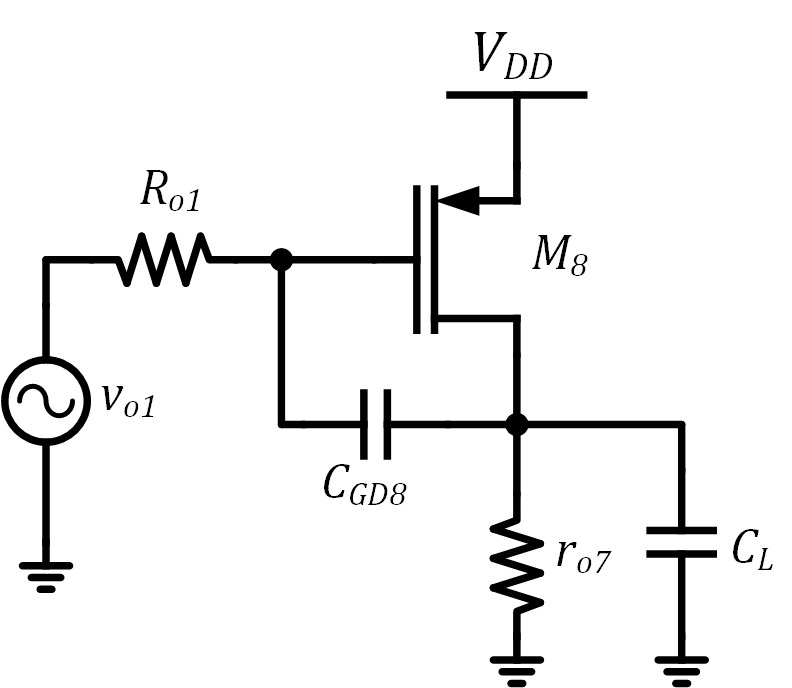
\includegraphics{2stage_OTA_simplified.png}
\caption{2stage\_OTA\_simplified.png}
\end{figure}

    \begin{itemize}
\tightlist
\item
  Assuming a ``large'' value of \(C_{GD}\), the two poles of the
  transfer function can be approximated as
\end{itemize}

\begin{equation}
\omega_{p1} \approx \dfrac{1}{R_{o1}(1+g_{m8} R_{o2})C_{GD}} 
\end{equation}

\begin{equation}
\omega_{p2} \approx \dfrac{g_{m8}C_{GD}}{C_{GD}(C_{GS}+C_L)+C_{GS}C_L}
\end{equation}

\begin{itemize}
\tightlist
\item
  The unity-gain frequency, \(\omega_u\) is approximately
\end{itemize}

\begin{align}
\omega_u \approx g_{m1}R_{o1}g_{m8}R_{o2} \cdot \dfrac{1}{g_{m8}R_{o2}R_{o1}C_{GD}} = \dfrac{g_{m1}}{C_{GD}}
\end{align}

\begin{itemize}
\tightlist
\item
  How do we guarantee a large enough value for \(C_{GD}\) to accomplish
  pole splitting?
\end{itemize}

    \hypertarget{miller-compensation}{%
\subsection{Miller compensation}\label{miller-compensation}}

    \begin{figure}
\centering
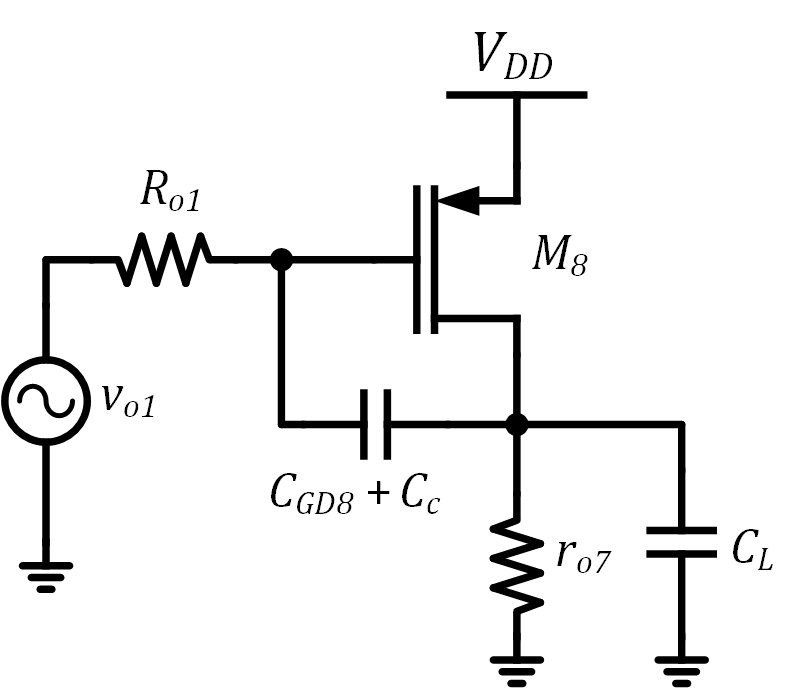
\includegraphics{2stage_OTA_simplified_Miller.png}
\caption{2stage\_OTA\_simplified\_Miller.png}
\end{figure}

    \begin{itemize}
\item
  We can add an explicit capacitance (e.g.~an integrated ``MIM''
  capacitor) to increase the effective value of \(C_{GD}\)
\item
  In general, \(C_c >> C_{GD}\), such that \(C_c + C_{GD} \approx C_c\)
\item
  Considering only \(\omega_{p1}\) and \(\omega_{p2}\) (ignoring
  \(\omega_{z}\), for the moment), the phase margin is given by
\end{itemize}

\begin{align}
PM &\approx 90^{\circ} - \tan^{-1}\dfrac{\omega_u}{\omega_{p2}}  \\
&= 90^{\circ} - \tan^{-1}\dfrac{g_{m1}(C_L + C_{GS8})}{g_{m8}C_{c}} \\
\end{align}

\begin{itemize}
\tightlist
\item
  Note that if \(C_L\) and \(C_c\) are comparable, \(g_{m8}\) should be
  much greater than \(g_{m1}\) to achieve a well-behaved response
\end{itemize}

    \begin{tcolorbox}[breakable, size=fbox, boxrule=1pt, pad at break*=1mm,colback=cellbackground, colframe=cellborder]
\prompt{In}{incolor}{7}{\boxspacing}
\begin{Verbatim}[commandchars=\\\{\}]
\PY{n}{gm1} \PY{o}{=} \PY{l+m+mf}{1e\PYZhy{}3}
\PY{n}{gm8} \PY{o}{=} \PY{l+m+mf}{1e\PYZhy{}3}
\PY{n}{ro} \PY{o}{=} \PY{l+m+mf}{100e3}
\PY{n}{R\PYZus{}o1} \PY{o}{=} \PY{n}{ro}\PY{o}{/}\PY{l+m+mi}{2} 
\PY{n}{R\PYZus{}o2} \PY{o}{=} \PY{n}{ro}\PY{o}{/}\PY{l+m+mi}{2}
\PY{n}{C\PYZus{}GD} \PY{o}{=} \PY{l+m+mf}{10e\PYZhy{}12}
\PY{n}{C\PYZus{}GS} \PY{o}{=} \PY{o}{.}\PY{l+m+mf}{2e\PYZhy{}12}
\PY{n}{C\PYZus{}L} \PY{o}{=} \PY{l+m+mf}{10e\PYZhy{}12}
\PY{n}{zeta} \PY{o}{=} \PY{n}{C\PYZus{}GS}\PY{o}{*}\PY{n}{C\PYZus{}GD} \PY{o}{+} \PY{n}{C\PYZus{}GS}\PY{o}{*}\PY{n}{C\PYZus{}L}\PY{o}{+}\PY{n}{C\PYZus{}GD}\PY{o}{*}\PY{n}{C\PYZus{}L}
\PY{n}{num} \PY{o}{=} \PY{p}{[}\PY{n}{C\PYZus{}GD}\PY{o}{*}\PY{n}{R\PYZus{}o2}\PY{o}{*}\PY{n}{gm1}\PY{o}{*}\PY{n}{R\PYZus{}o1}\PY{p}{,} \PY{o}{\PYZhy{}}\PY{n}{gm8}\PY{o}{*}\PY{n}{R\PYZus{}o2}\PY{o}{*}\PY{n}{gm1}\PY{o}{*}\PY{n}{R\PYZus{}o1}\PY{p}{]}
\PY{n}{den} \PY{o}{=} \PY{p}{[}\PY{n}{R\PYZus{}o1}\PY{o}{*}\PY{n}{R\PYZus{}o2}\PY{o}{*}\PY{n}{zeta}\PY{p}{,} \PY{n}{gm1}\PY{o}{*}\PY{n}{R\PYZus{}o1}\PY{o}{*}\PY{n}{R\PYZus{}o2}\PY{o}{*}\PY{n}{C\PYZus{}GD}\PY{o}{+}\PY{n}{R\PYZus{}o1}\PY{o}{*}\PY{n}{C\PYZus{}GS}\PY{o}{+}\PY{n}{R\PYZus{}o2}\PY{o}{*}\PY{p}{(}\PY{n}{C\PYZus{}GD}\PY{o}{+}\PY{n}{C\PYZus{}L}\PY{p}{)}\PY{p}{,} \PY{l+m+mi}{1}\PY{p}{]}
\PY{n}{tf\PYZus{}CS} \PY{o}{=} \PY{n}{signal}\PY{o}{.}\PY{n}{TransferFunction}\PY{p}{(}\PY{o}{\PYZhy{}}\PY{n}{gm1}\PY{o}{*}\PY{n}{R\PYZus{}o1}\PY{o}{*}\PY{n}{gm8}\PY{o}{*}\PY{n}{R\PYZus{}o2}\PY{p}{,}  \PY{n}{den}\PY{p}{)}
\PY{n}{w}\PY{p}{,} \PY{n}{mag}\PY{p}{,} \PY{n}{phase} \PY{o}{=} \PY{n}{tf\PYZus{}CS}\PY{o}{.}\PY{n}{bode}\PY{p}{(}\PY{p}{)}       
\PY{n}{f} \PY{o}{=} \PY{n}{w}\PY{o}{/}\PY{l+m+mi}{2}\PY{o}{/}\PY{n}{np}\PY{o}{.}\PY{n}{pi}  
\end{Verbatim}
\end{tcolorbox}

    \begin{tcolorbox}[breakable, size=fbox, boxrule=1pt, pad at break*=1mm,colback=cellbackground, colframe=cellborder]
\prompt{In}{incolor}{8}{\boxspacing}
\begin{Verbatim}[commandchars=\\\{\}]
\PY{n}{plot\PYZus{}logxy2}\PY{p}{(}\PY{n}{f}\PY{p}{,} \PY{n}{mag}\PY{p}{,} \PY{n}{f}\PY{p}{,} \PY{n}{phase}\PY{p}{,} \PY{l+s+s1}{\PYZsq{}}\PY{l+s+s1}{Frequency [Hz]}\PY{l+s+s1}{\PYZsq{}}\PY{p}{,} \PY{l+s+s1}{\PYZsq{}}\PY{l+s+s1}{Magnitude [dB]}\PY{l+s+s1}{\PYZsq{}}\PY{p}{,}
           \PY{l+s+s1}{\PYZsq{}}\PY{l+s+s1}{Frequency [Hz]}\PY{l+s+s1}{\PYZsq{}}\PY{p}{,} \PY{l+s+s1}{\PYZsq{}}\PY{l+s+s1}{Phase [deg]}\PY{l+s+s1}{\PYZsq{}}\PY{p}{)}
\end{Verbatim}
\end{tcolorbox}

    \begin{center}
    \adjustimage{max size={0.9\linewidth}{0.9\paperheight}}{2021_03_03_EE538_Lecture9_W2021_files/2021_03_03_EE538_Lecture9_W2021_17_0.png}
    \end{center}
    { \hspace*{\fill} \\}
    
    \begin{itemize}
\item
  Even without the influence of \(\omega_z\), the phase margin is only
  about \(45^{\circ}\)
\item
  What happens when we consider \(\omega_z\)?
\end{itemize}

    \hypertarget{effect-of-the-rhp-zero-on-phase-margin}{%
\subsection{Effect of the RHP zero on phase
margin}\label{effect-of-the-rhp-zero-on-phase-margin}}

    \begin{itemize}
\tightlist
\item
  The expression in the numerator,
  \(N(j\omega) = (sC_{c} - g_{m8})R_{o2}\) results in a zero in the
  right half of the complex plane
\end{itemize}

\begin{equation} 
\omega_z = \dfrac{g_{m8}}{C_{c}}
\end{equation}

\begin{itemize}
\tightlist
\item
  A zero in the right-half plane increases phase lag as well as gain
  magnitude, which can be detrimental to stability
\end{itemize}

\begin{align}
PM &\approx 90^{\circ} - \tan^{-1}\dfrac{\omega_u}{\omega_{p2}} - \tan^{-1}\dfrac{\omega_u}{\omega_{z}} \\
\\
&= 90^{\circ} - \tan^{-1}\dfrac{g_{m1}C_L}{g_{m8}C_{c}} - \tan^{-1}\dfrac{g_{m1}}{g_{m8}}\\
\end{align}

\begin{itemize}
\tightlist
\item
  The phase lag due to \(\omega_z\) can be up to \(45^{\circ}\) (or
  greater) if \(g_{m1}\) and \(g_{m8}\) are comparable
\end{itemize}

    \begin{tcolorbox}[breakable, size=fbox, boxrule=1pt, pad at break*=1mm,colback=cellbackground, colframe=cellborder]
\prompt{In}{incolor}{9}{\boxspacing}
\begin{Verbatim}[commandchars=\\\{\}]
\PY{n}{gm1} \PY{o}{=} \PY{l+m+mf}{1e\PYZhy{}3}
\PY{n}{gm8} \PY{o}{=} \PY{l+m+mf}{1e\PYZhy{}3}
\PY{n}{ro} \PY{o}{=} \PY{l+m+mf}{100e3}
\PY{n}{R\PYZus{}o1} \PY{o}{=} \PY{n}{ro}\PY{o}{/}\PY{l+m+mi}{2} 
\PY{n}{R\PYZus{}o2} \PY{o}{=} \PY{n}{ro}\PY{o}{/}\PY{l+m+mi}{2}
\PY{n}{C\PYZus{}GD} \PY{o}{=} \PY{l+m+mf}{10e\PYZhy{}12}
\PY{n}{C\PYZus{}GS} \PY{o}{=} \PY{o}{.}\PY{l+m+mf}{2e\PYZhy{}12}
\PY{n}{C\PYZus{}L} \PY{o}{=} \PY{l+m+mf}{10e\PYZhy{}12}
\PY{n}{zeta} \PY{o}{=} \PY{n}{C\PYZus{}GS}\PY{o}{*}\PY{n}{C\PYZus{}GD} \PY{o}{+} \PY{n}{C\PYZus{}GS}\PY{o}{*}\PY{n}{C\PYZus{}L}\PY{o}{+}\PY{n}{C\PYZus{}GD}\PY{o}{*}\PY{n}{C\PYZus{}L}
\PY{n}{num} \PY{o}{=} \PY{p}{[}\PY{n}{C\PYZus{}GD}\PY{o}{*}\PY{n}{R\PYZus{}o2}\PY{o}{*}\PY{n}{gm1}\PY{o}{*}\PY{n}{R\PYZus{}o1}\PY{p}{,} \PY{o}{\PYZhy{}}\PY{n}{gm8}\PY{o}{*}\PY{n}{R\PYZus{}o2}\PY{o}{*}\PY{n}{gm1}\PY{o}{*}\PY{n}{R\PYZus{}o1}\PY{p}{]}
\PY{n}{den} \PY{o}{=} \PY{p}{[}\PY{n}{R\PYZus{}o1}\PY{o}{*}\PY{n}{R\PYZus{}o2}\PY{o}{*}\PY{n}{zeta}\PY{p}{,} \PY{n}{gm1}\PY{o}{*}\PY{n}{R\PYZus{}o1}\PY{o}{*}\PY{n}{R\PYZus{}o2}\PY{o}{*}\PY{n}{C\PYZus{}GD}\PY{o}{+}\PY{n}{R\PYZus{}o1}\PY{o}{*}\PY{n}{C\PYZus{}GS}\PY{o}{+}\PY{n}{R\PYZus{}o2}\PY{o}{*}\PY{p}{(}\PY{n}{C\PYZus{}GD}\PY{o}{+}\PY{n}{C\PYZus{}L}\PY{p}{)}\PY{p}{,} \PY{l+m+mi}{1}\PY{p}{]}
\PY{n}{tf\PYZus{}CS} \PY{o}{=} \PY{n}{signal}\PY{o}{.}\PY{n}{TransferFunction}\PY{p}{(}\PY{n}{num}\PY{p}{,}  \PY{n}{den}\PY{p}{)}
\PY{n}{w}\PY{p}{,} \PY{n}{mag}\PY{p}{,} \PY{n}{phase} \PY{o}{=} \PY{n}{tf\PYZus{}CS}\PY{o}{.}\PY{n}{bode}\PY{p}{(}\PY{p}{)}       
\PY{n}{f} \PY{o}{=} \PY{n}{w}\PY{o}{/}\PY{l+m+mi}{2}\PY{o}{/}\PY{n}{np}\PY{o}{.}\PY{n}{pi}  
\end{Verbatim}
\end{tcolorbox}

    \begin{tcolorbox}[breakable, size=fbox, boxrule=1pt, pad at break*=1mm,colback=cellbackground, colframe=cellborder]
\prompt{In}{incolor}{10}{\boxspacing}
\begin{Verbatim}[commandchars=\\\{\}]
\PY{n}{plot\PYZus{}logxy2}\PY{p}{(}\PY{n}{f}\PY{p}{,} \PY{n}{mag}\PY{p}{,} \PY{n}{f}\PY{p}{,} \PY{n}{phase}\PY{p}{,} \PY{l+s+s1}{\PYZsq{}}\PY{l+s+s1}{Frequency [Hz]}\PY{l+s+s1}{\PYZsq{}}\PY{p}{,} \PY{l+s+s1}{\PYZsq{}}\PY{l+s+s1}{Magnitude [dB]}\PY{l+s+s1}{\PYZsq{}}\PY{p}{,}
           \PY{l+s+s1}{\PYZsq{}}\PY{l+s+s1}{Frequency [Hz]}\PY{l+s+s1}{\PYZsq{}}\PY{p}{,} \PY{l+s+s1}{\PYZsq{}}\PY{l+s+s1}{Phase [deg]}\PY{l+s+s1}{\PYZsq{}}\PY{p}{)}
\end{Verbatim}
\end{tcolorbox}

    \begin{center}
    \adjustimage{max size={0.9\linewidth}{0.9\paperheight}}{2021_03_03_EE538_Lecture9_W2021_files/2021_03_03_EE538_Lecture9_W2021_22_0.png}
    \end{center}
    { \hspace*{\fill} \\}
    
    \begin{itemize}
\item
  Here, the phase margin has decreased to zero with the inclusion of
  \(\omega_z\)
\item
  The effect isn't evident from the magnitude response alone, since the
  rolloff from \(\omega_{p2}\) is countered by a \(20dB/dec\)
  \emph{increase} in the magnitude due to \(\omega_z\)
\item
  How do we improve the phase margin?
\end{itemize}

    \hypertarget{moving-the-rhp-zero}{%
\subsection{Moving the RHP zero}\label{moving-the-rhp-zero}}

    \begin{figure}
\centering
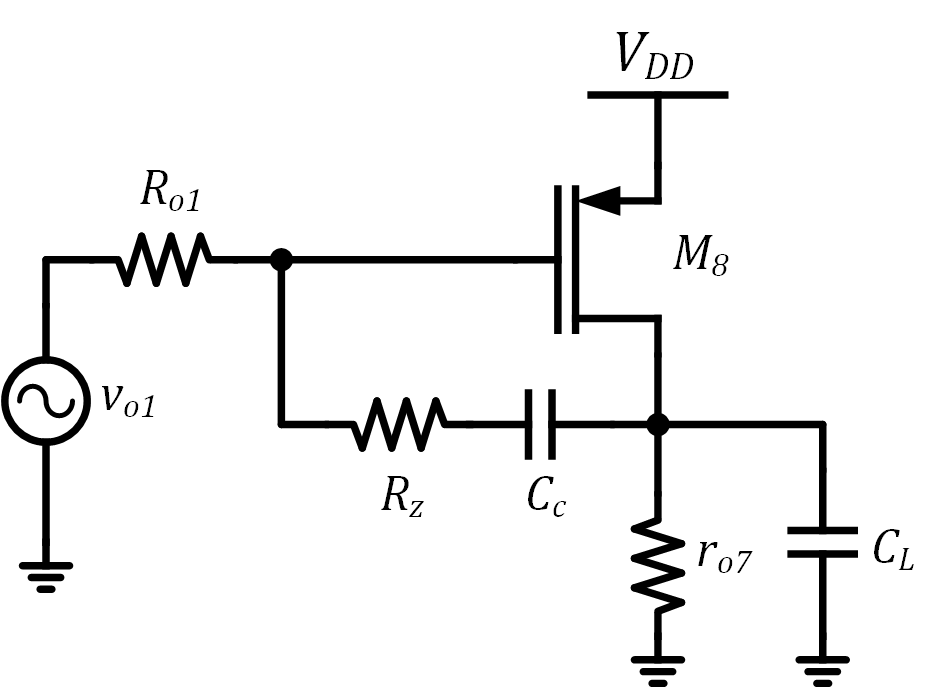
\includegraphics{2stage_OTA_simplified_Rz.png}
\caption{2stage\_OTA\_simplified\_Rz.png}
\end{figure}

    \begin{itemize}
\item
  We can manipulate \(\omega_z\) by inserting a resistor, \(R_z\), in
  series with \(C_c\)
\item
  Properly chosen, \(R_z\) can eliminate the RHP zero altogether
  (pushing it to ``infinite'' frequency)
\item
  This isn't achievable in practice, since neither \(g_{m8}\) nor
  \(R_z\) is precisely defined (due to variations in process and
  temperature)
\item
  We can instead move \(\omega_z\) to the LHP, transforming phase lag
  into lead
\end{itemize}

    \begin{itemize}
\tightlist
\item
  With the inclusion of \(R_z\) the expression for the zero becomes
\end{itemize}

\begin{equation} 
\omega_z = \dfrac{1}{C_{c}(g_{m8}^{-1} - R_z)}
\end{equation}

\begin{itemize}
\item
  Using \(R_z = 1/g_{m8}\) effectively ``cancels'' \(\omega_z\), pushing
  to it to infinity
\item
  A more reliable approach is to use \(R_z > 1/g_{m8}\) to move
  \(\omega_z\) to the left-half of the complex plane
\item
  What is a reasonable choice for the value of \(R_z\)?
\end{itemize}

    \hypertarget{non-dominant-pole-cancellation}{%
\subsection{Non-dominant pole
cancellation}\label{non-dominant-pole-cancellation}}

    \begin{itemize}
\tightlist
\item
  The modified zero location is given by
\end{itemize}

\begin{equation} 
\omega_z = \dfrac{1}{C_{c}(g_{m8}^{-1} - R_z)}
\end{equation}

\begin{itemize}
\tightlist
\item
  If we design \(R_z\) to achieve \(\omega_{z,LHP} = \omega_{p1}\), this
  results in a value of \(R_z\) given by
\end{itemize}

\begin{equation}
\omega_z = \dfrac{1}{C_{c}(g_{m8}^{-1} - R_z)} = \dfrac{g_{m8}}{C_L + C_{GD8}} = \omega_{p1} \rightarrow \boxed{R_z = \dfrac{C_L + C_c + C_{GS8}}{g_{m8} C_c}}
\end{equation}

\begin{itemize}
\item
  Moving \(\omega_z\) to overlap with \(\omega_{p2}\) accomplishes two
  things:

  \begin{enumerate}
  \def\labelenumi{\arabic{enumi}.}
  \item
    Removes the phase lag of the RHP zero
    (\(\omega_{z,RHP} \rightarrow \omega_{z,LHP}\))
  \item
    Reduces/eliminates the phase lag due to the non-dominant pole
    \(w_{p2}\)
  \end{enumerate}
\end{itemize}

    \hypertarget{variability-in-gm2rz}{%
\subsection{Variability in Gm2Rz}\label{variability-in-gm2rz}}

    \begin{figure}
\centering
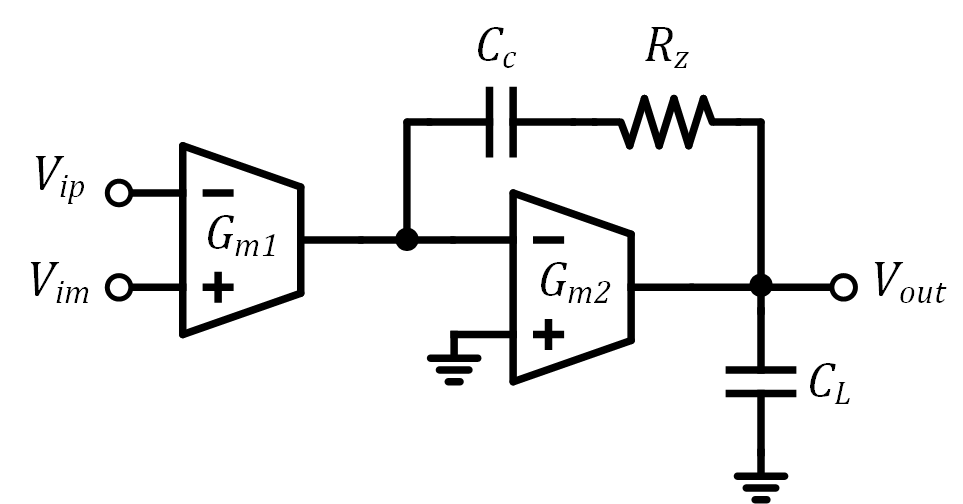
\includegraphics{2stage_compensated.png}
\caption{2stage\_compensated.png}
\end{figure}

    \begin{itemize}
\item
  To maximize PM we want \(R_z \approx \dfrac{C_L + C_c}{G_{m2} C_c}\)
\item
  If \(\dfrac{C_L + C_c}{C_c}\) is constant, we want
\end{itemize}

\begin{equation}
G_{m2}R_z = \dfrac{C_L + C_c}{C_c} = constant
\end{equation}

    \begin{itemize}
\tightlist
\item
  Unfortunately, \(G_{m2}\) and \(R_z\) don't track each other in terms
  of process and temperature variations
\item
  However, if we could somehow define \(G_{m2}\) in terms of a
  resistance that varies in a similar manner to \(R_z\), we could remove
  this source of uncertainty
\end{itemize}

    \hypertarget{constant-gm-reference}{%
\subsection{Constant-Gm reference}\label{constant-gm-reference}}

    \begin{itemize}
\tightlist
\item
  If the second stage (\(G_{m2}\)) is biased using a constant-\(g_m\)
  reference, variations in \(R_z\) due to process and temperature can be
  tracked by \(G_{m2}\)
\item
  In this case, both \(R_z\) and \(R_s\) should be implemented on chip
  using the same type of resistor
\item
  Biasing in this manner results in
\end{itemize}

\begin{equation}
G_{m2} = \dfrac{K_2}{2\cdot R_S}
\end{equation}

\begin{itemize}
\tightlist
\item
  Note that \(g_m/I_D\) should be the same for \(M_1\) of the reference
  and the input pair of \(G_{m2}\)
\end{itemize}

    \begin{figure}
\centering
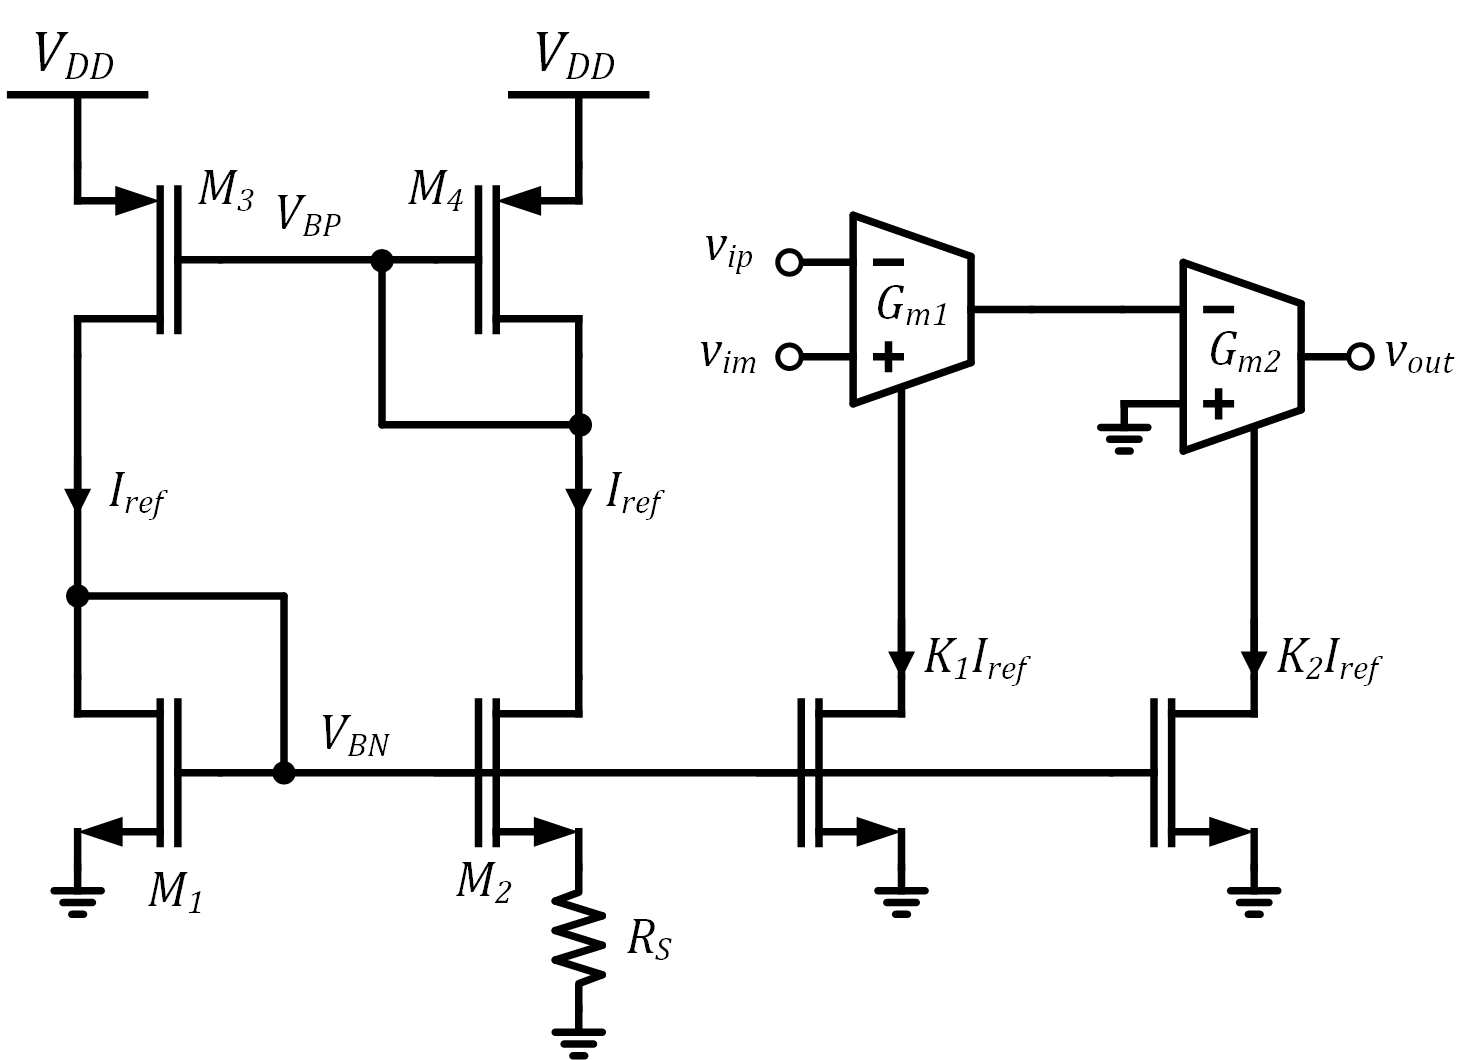
\includegraphics{constant_Gm.png}
\caption{constant\_Gm.png}
\end{figure}

    \hypertarget{pole-zero-doublet-problem}{%
\subsection{Pole-zero doublet problem}\label{pole-zero-doublet-problem}}

    \begin{figure}
\centering
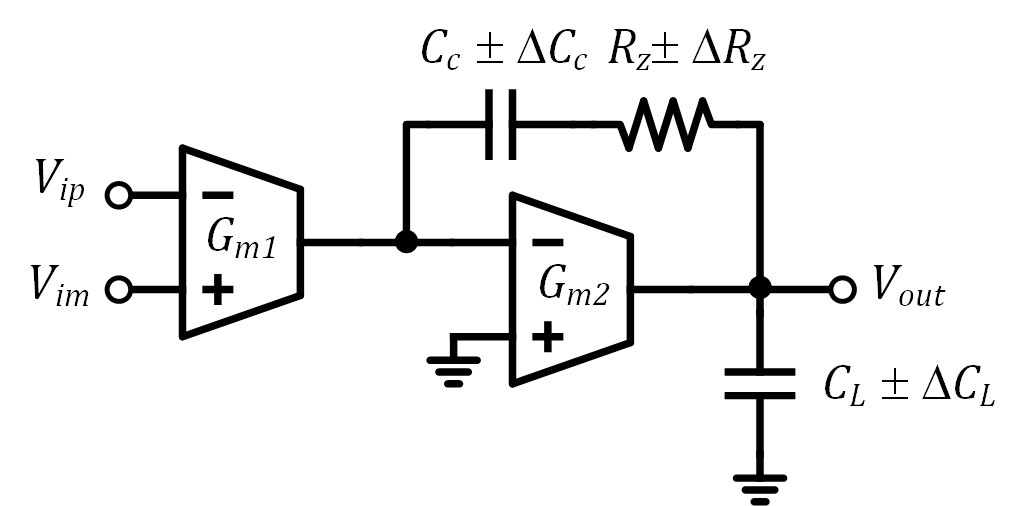
\includegraphics{2stage_OTA_component_variability.png}
\caption{2stage\_OTA\_component\_variability.png}
\end{figure}

    \begin{itemize}
\item
  The possibility of canceling the non-dominant pole is attractive, but
  in practice cancellation is imperfect
\item
  It cannot be guaranteed that \(\omega_z = \omega_{p2}\), due to
  variations in \(G_{m2}\), \(R_z\), \(C_c\), and \(C_L\)
\item
  Mismatch in the frequencies of \(\omega_z\) and \(\omega_{p2}\)
  results in a phenomenon known as a pole-zero ``doublet,'' which can
  significantly degrade the settling time of the OTA (particularly
  important for switched-capacitor applications)
\end{itemize}

    \hypertarget{an-alternate-approach-ahuja-compensation}{%
\subsection{An alternate approach (Ahuja
compensation)}\label{an-alternate-approach-ahuja-compensation}}

    \begin{itemize}
\item
  The feedforward path can be eliminated by the addition of a
  common-gate stage (\(M_2\)) in the feedback path
\item
  The common-gate stage effectively multiplies the transconductance of
  \(M_1\) by the common-gate stage gain, which is approximately
  \(g_{m2} R_{o1}\)
\item
  The transfer function contains a zero in the \emph{left half plane},
  which can similarly be used to manipulate phase lag due to
  \(\omega_{p2}\)
\item
  This structure has the additional benefit of tolerance to larger
  values of \(C_L\), since the non-dominant pole becomes (approximately)
\end{itemize}

\begin{equation}
\omega_{p2} \approx \dfrac{g_{m2}R_{o1}g_{m1}}{C_L}
\end{equation}

    \begin{figure}
\centering
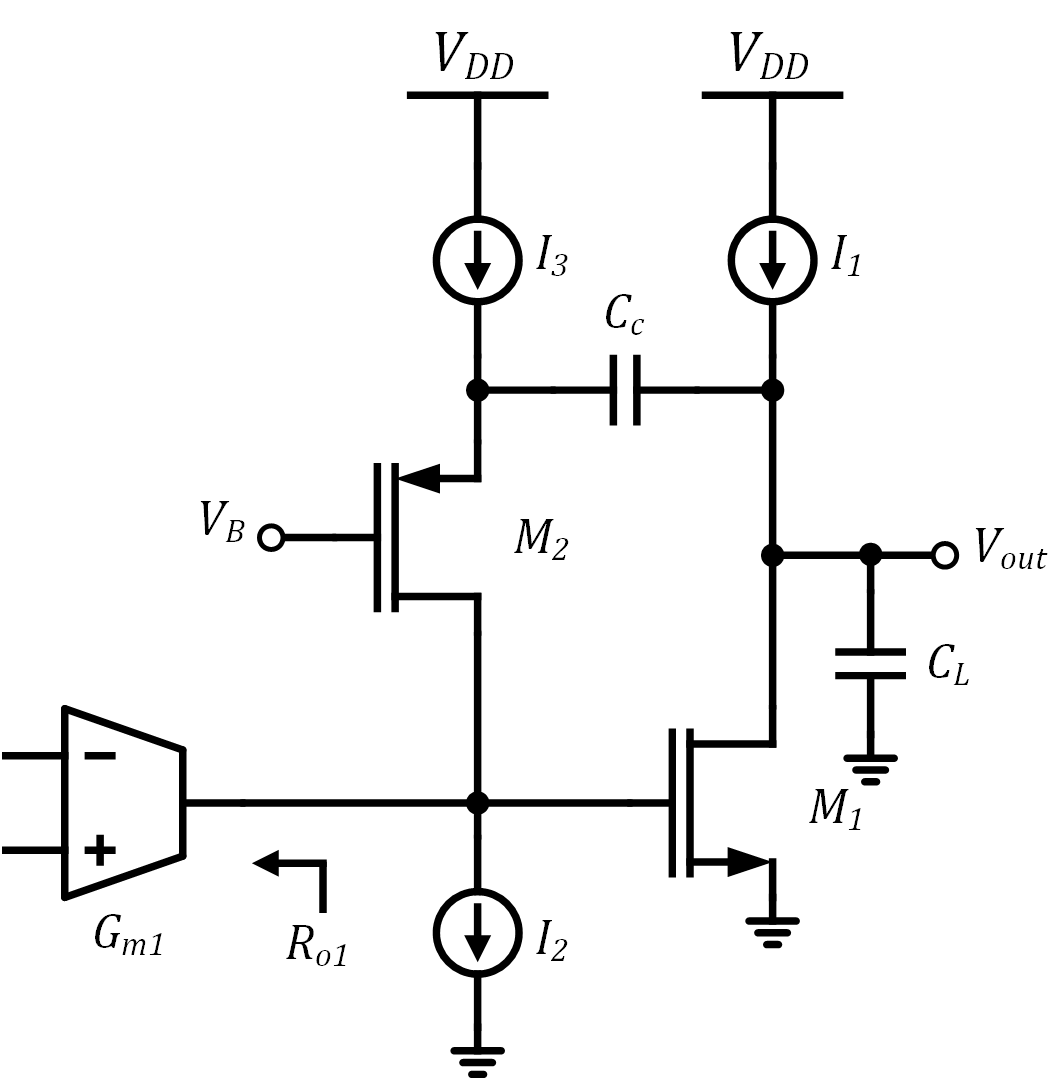
\includegraphics{Ahuja_compensation.png}
\caption{Ahuja\_compensation.png}
\end{figure}

    \hypertarget{common-gate-stage}{%
\subsection{Common-gate stage}\label{common-gate-stage}}

    \begin{figure}
\centering
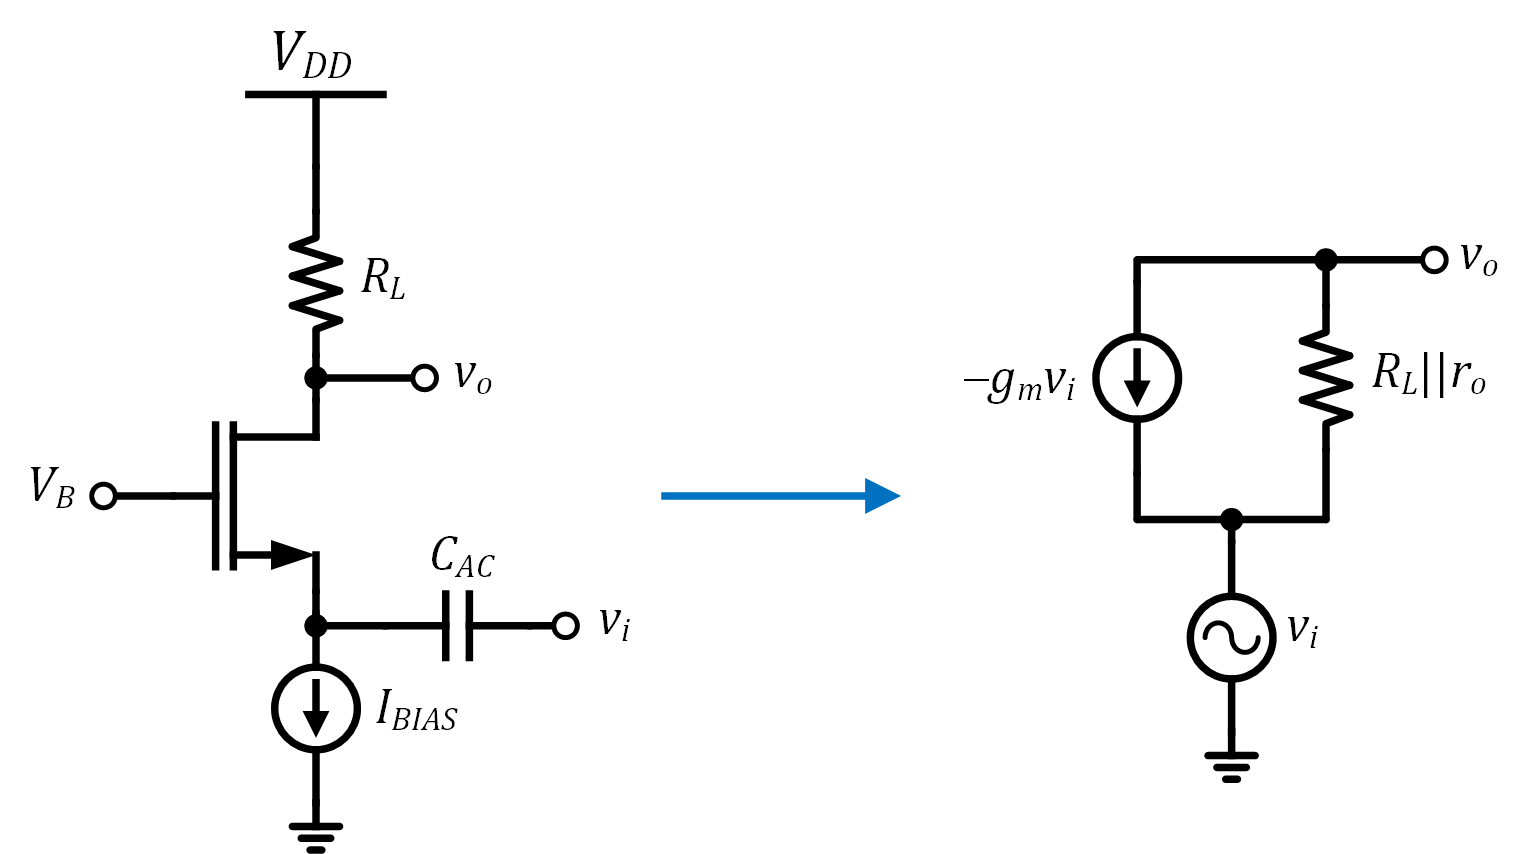
\includegraphics{common_gate_stage.png}
\caption{common\_gate\_stage.png}
\end{figure}

    \begin{itemize}
\tightlist
\item
  The common-gate stage is often used as a current-input
  (transimpedance) amplifier, in addition to being an instrinsic
  structure in the cascode amplifier
\item
  The voltage gain is the same as that of a common-source stage, but it
  is non-inverting
\end{itemize}

    \begin{figure}
\centering
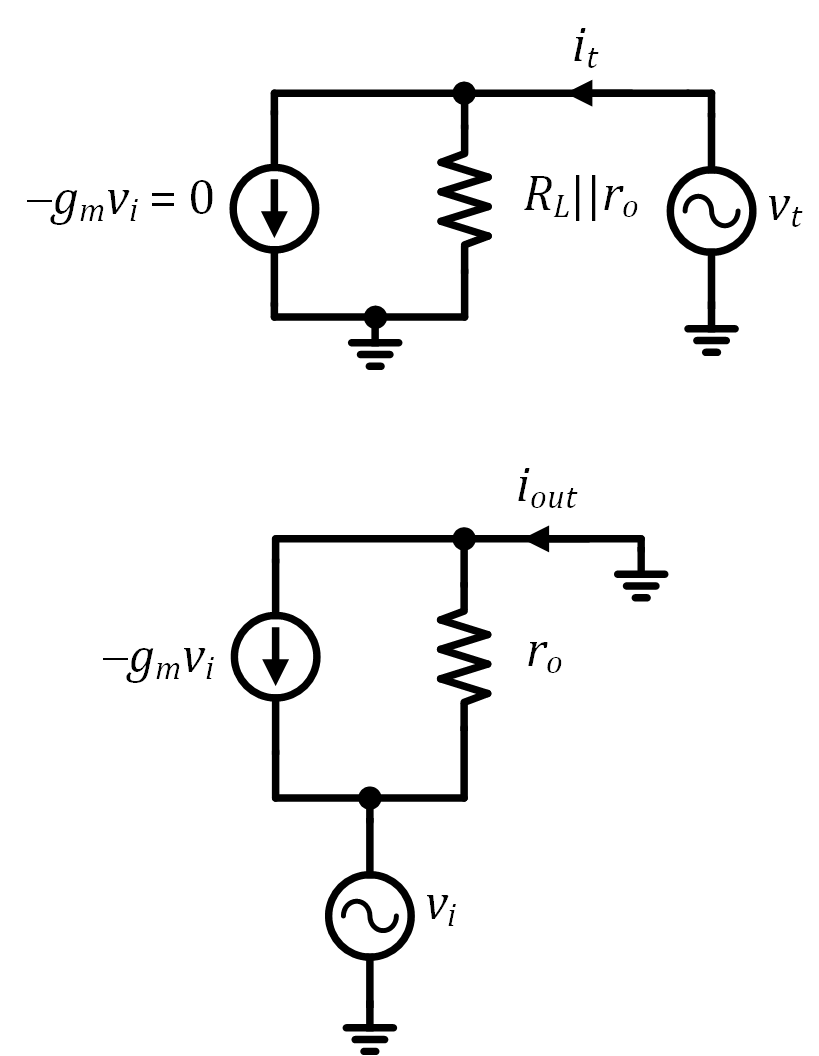
\includegraphics{common_gate_Ro.png}
\caption{common\_gate\_Ro.png}
\end{figure}

    \begin{itemize}
\tightlist
\item
  As with other structures, \(R_o\) is determined by setting
  \(v_i \rightarrow 0\) and finding \(v_t/i_t\)
\end{itemize}

\begin{equation}
R_o = \dfrac{v_t}{i_t} = R_L||r_o
\end{equation}

\begin{itemize}
\tightlist
\item
  \(G_m\) can be found by shorting the output to ground and
  ``measuring'' the output current
\end{itemize}

\begin{equation}
i_{out} = -g_m v_i - \dfrac{v_i}{r_o}
\end{equation}

\begin{equation}
G_m = \dfrac{i_{out}}{v_i} = -g_m - \dfrac{1}{r_o}
\end{equation}

\begin{itemize}
\tightlist
\item
  The voltage gain of the common-gate stage is given by
\end{itemize}

\begin{equation}
\boxed{\dfrac{v_o}{v_i} = -G_m R_o \approx g_m(R_L||r_o)} 
\end{equation}

    \hypertarget{gain-boosting}{%
\subsection{Gain boosting}\label{gain-boosting}}

    \begin{itemize}
\item
  Gain-boosting can be used to enhance the effective transconductance of
  \(M_{2}\) and \(M_{3}\) and increase output impedance
\item
  \(U_{1,2}\) amplify the small-signal voltages at \(v_{s2}\) and
  \(v_{s3}\) to boost the small-signal transconductance currents of
  \(M_2\) and \(M_3\)
\item
  \(U_1\) and \(U_2\) can be implemented as single-stage OTA's with or
  without cascoding
\item
  If \(U_{1,2}\) are cascode amplifiers (with DC gain
  \(\propto g_m^2 r_o^2\)), the gain of the primary amplifier can be
  increased to
\end{itemize}

\begin{equation}
|A_{v0}| = G_m R_o \propto g_m^4 r_o^4
\end{equation}

\begin{itemize}
\tightlist
\item
  Bias voltages \(V_{BN}\) and \(V_{BP1}\) should be
  \(V_{GS2}\)/\(V_{SG3}\) lower/higher than the target gate bias
\end{itemize}

    \begin{figure}
\centering
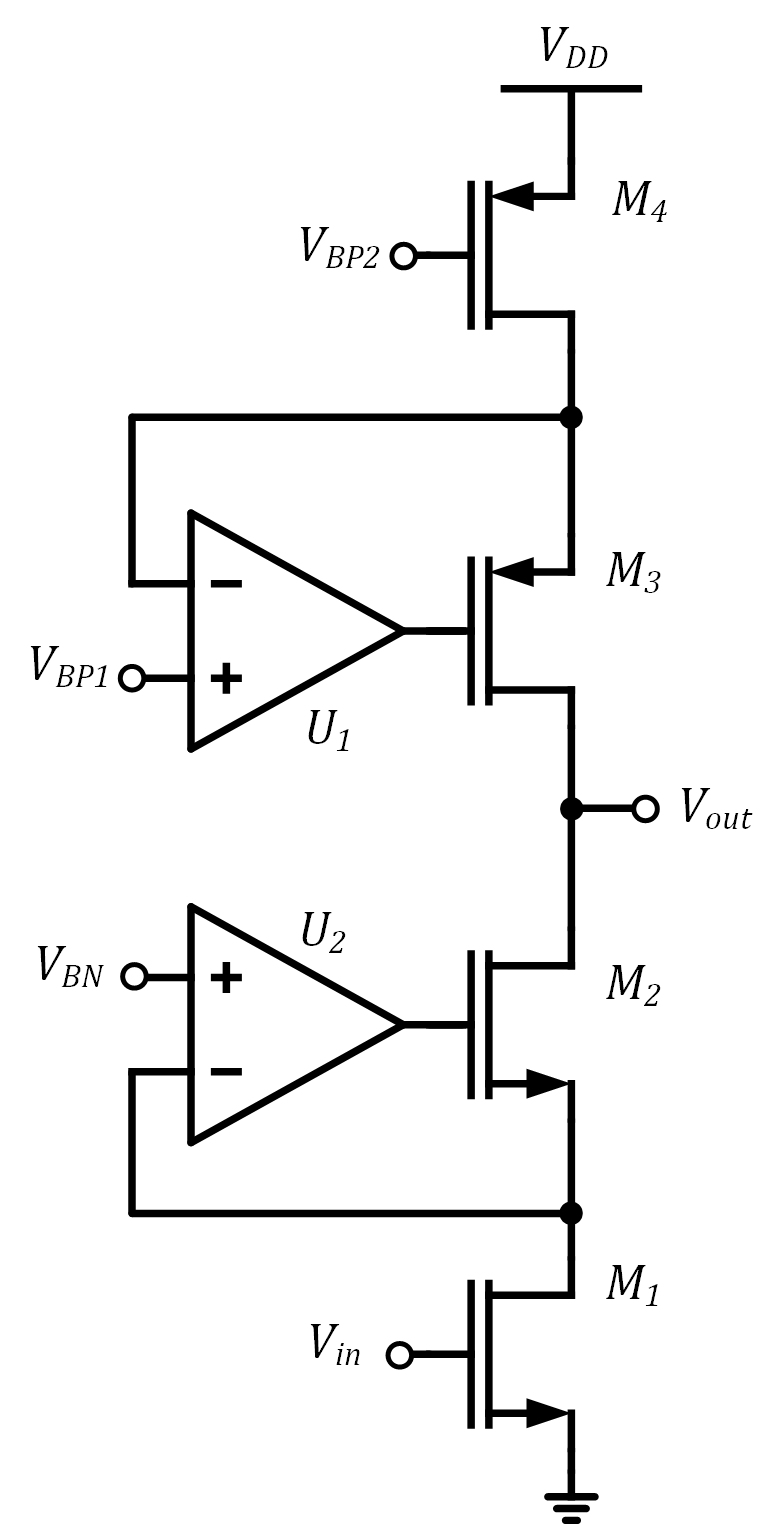
\includegraphics{gain_boosted_cascode.png}
\caption{gain\_boosted\_cascode.png}
\end{figure}

    \begin{figure}
\centering
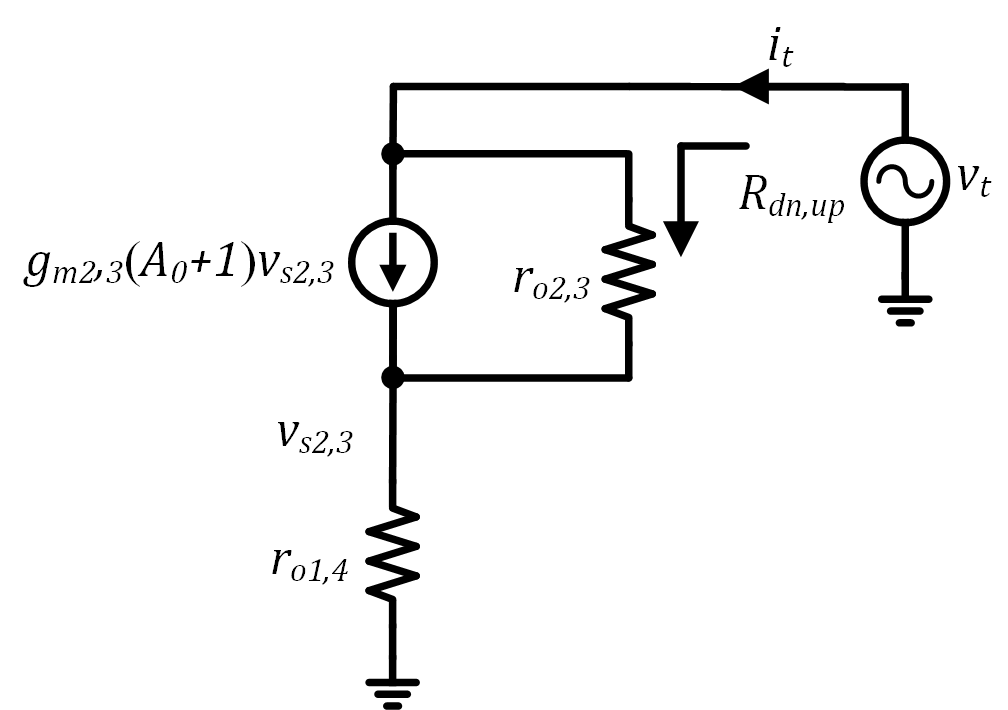
\includegraphics{Ro_boosted_half_circuit.png}
\caption{Ro\_boosted\_half\_circuit.png}
\end{figure}

    \begin{itemize}
\item
  \(A_0\) is the open-loop gain of the auxiliary amplifiers \(U_1\) and
  \(U_2\)
\item
  KCL for the half-circuit (plus Ohm's law for \(r_{o1}\)) gives
\end{itemize}

\begin{equation}
i_t = g_{m2,3}(A_0+1)v_{s} + \dfrac{v_t - v_s}{r_{o2,3}} = \dfrac{v_s}{r_{o1}}
\end{equation}

\begin{itemize}
\tightlist
\item
  This results in a half-circuit impedance of
\end{itemize}

\begin{equation}
\dfrac{v_t}{i_t} = r_{o2,3} + r_{o1,4} + g_{m2,3} r_{o2,3}r_{o1,4}(A_0+1)
\end{equation}

\begin{itemize}
\tightlist
\item
  The parallel combination of the two halves is given approximately by
\end{itemize}

\begin{equation}
R_o \approx \left[ g_{m2} r_{o1}r_{o2}A_0 \right] || \left[ g_{m3}r_{o3}r_{o4}A_0 \right] 
\end{equation}

    \hypertarget{implementation-of-u12}{%
\subsection{Implementation of U1,2}\label{implementation-of-u12}}

    \begin{figure}
\centering
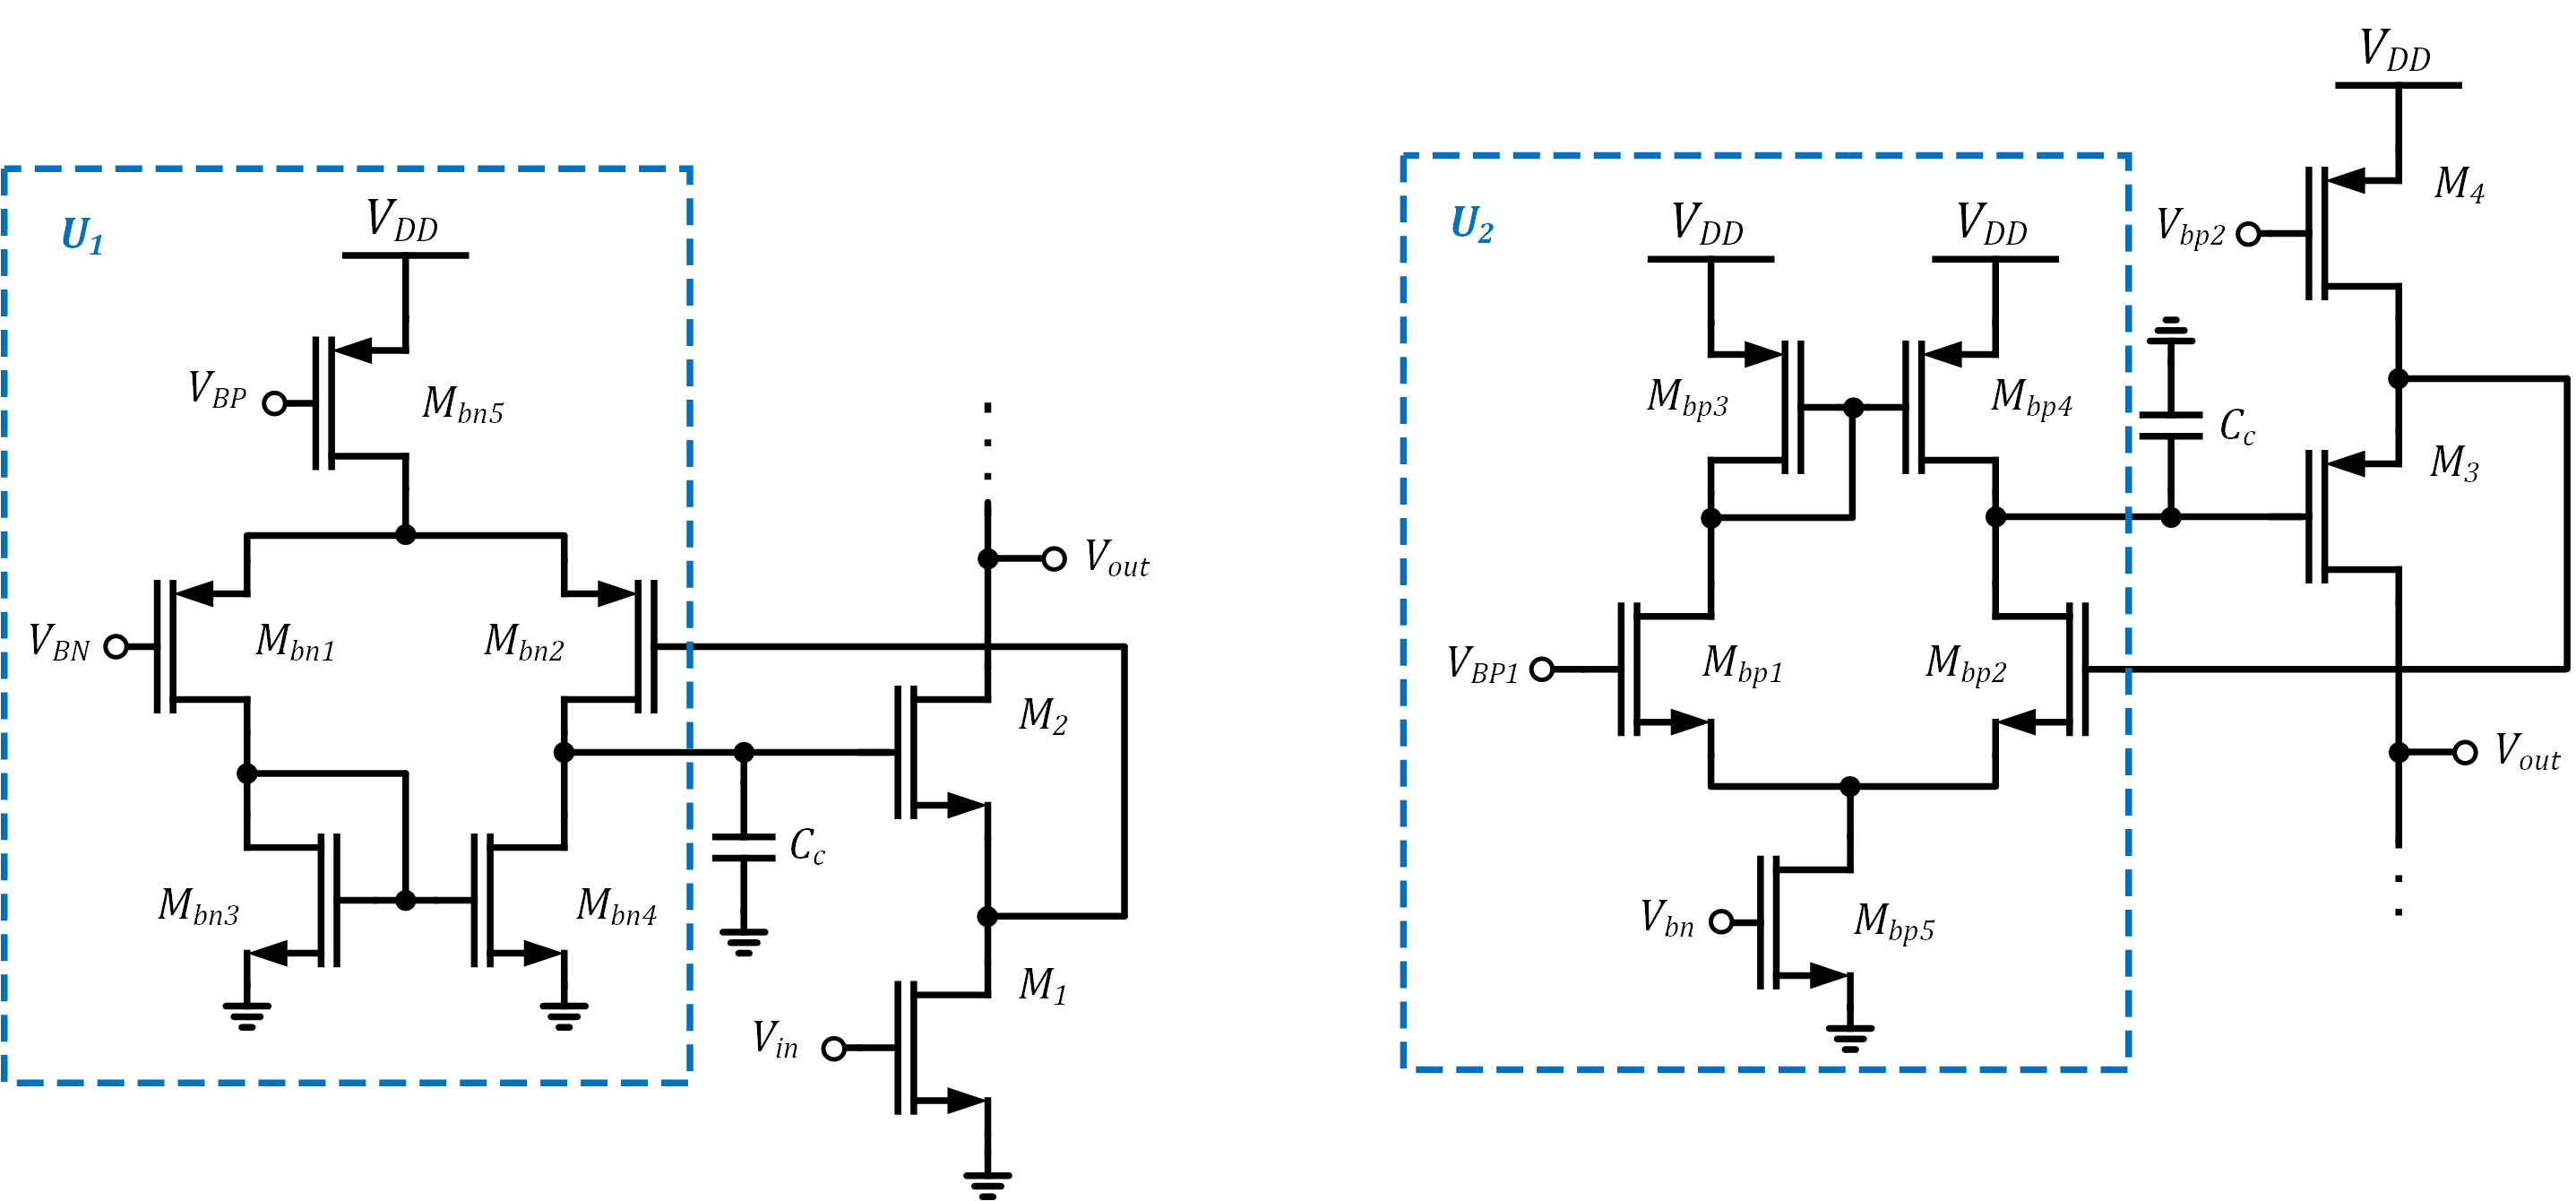
\includegraphics{gain_boosting_OTAs.png}
\caption{gain\_boosting\_OTAs.png}
\end{figure}

    \begin{itemize}
\tightlist
\item
  One means of generating the regulated cascode bias is shown here

  \begin{itemize}
  \tightlist
  \item
    \(U_{1,2}\) should be compensated to ensure stability of the local
    feedback
  \item
    This can be accomplished by placing a compensation capacitor
    (\(C_c\)) between the auxiliary OTA output and small-signal ground,
    putting the frequency of the dominant pole at
    \(\omega_{0,boost} \approx \dfrac{2}{r_o C_c}\)
  \end{itemize}
\end{itemize}

    \hypertarget{summary}{%
\subsection{Summary}\label{summary}}

    \begin{itemize}
\tightlist
\item
  2-stage CMOS OTA's are typically compensated by increasing the Miller
  capacitance of the second stage to make the Miller pole dominant
\item
  Miller compensation produces a non-dominant pole at approximately
  \(\omega_{p2} = G_{m2}/C_L\) and a RHP zero at
  \(\omega_z = G_{m2}/C_c\)
\item
  To alleviate the phase lag due to \(\omega_{p2}\) and \(\omega_{z}\),
  \(\omega_{z}\) can be moved to the LHP, close in frequency to
  \(\omega_{p2}\)
\item
  In practice, cancellation is imperfect and can result in slow setting
  (pole-zero doublet)
\item
  Gain-boosting is an alternative to the 2-stage design that is simpler
  to compensate but adds complexity due to the required auxiliary
  amplifiers
\item
  Gain-boosting results in lower output swing, so a folded cascode is
  often preferred
\end{itemize}


    % Add a bibliography block to the postdoc
    
    
    
\end{document}
